%---------------------------------------------
%	7. Application & Perform of GNN Algorithm
%---------------------------------------------

\chapter{Application of the GNN Algorithm to the TrackML Model}
\label{chapter-7}

This chapter focuses on the application of the GNN algorithm to the Pixel endcap and Pixel barrel regions of the TrackML detector. This chapter is organised as follows. Section \ref{chapter-7-endcap-results} presents the results of the GNN algorithm applied to the Pixel endcap region of the TrackML detector. The performance of the algorithm is evaluated and track reconstruction efficiency metrics are discussed. Section \ref{chapter-7-outlook} presents an outlook to the future of this research. Preliminary results and challenges faced when applying the GNN algorithm onto the entire Pixel detector of the TrackML geometry, including the Pixel barrel region, are presented. Potential software optimisations and other approaches explored are also discussed, followed by several improvements that would be necessary to implement within the GNN algorithm for track reconstruction in particle detectors.





\section{Pixel Endcap Results}
\label{chapter-7-endcap-results}

The GNN algorithm is first applied to volume 7 of the TrackML detector model, by isolating the left Pixel endcap. The geometry in the endcap consists of parallel silicon layers and is the simplest part of the detector to begin reconstruction. An example TrackML simulated event shown in volume 7 can be seen in Figure \ref{fig:trackml-results-endcap-nodes-sim}.

\begin{figure}[htbp!] 
    \centering
    \subfloat[$x$-$y$ plane view]{%
        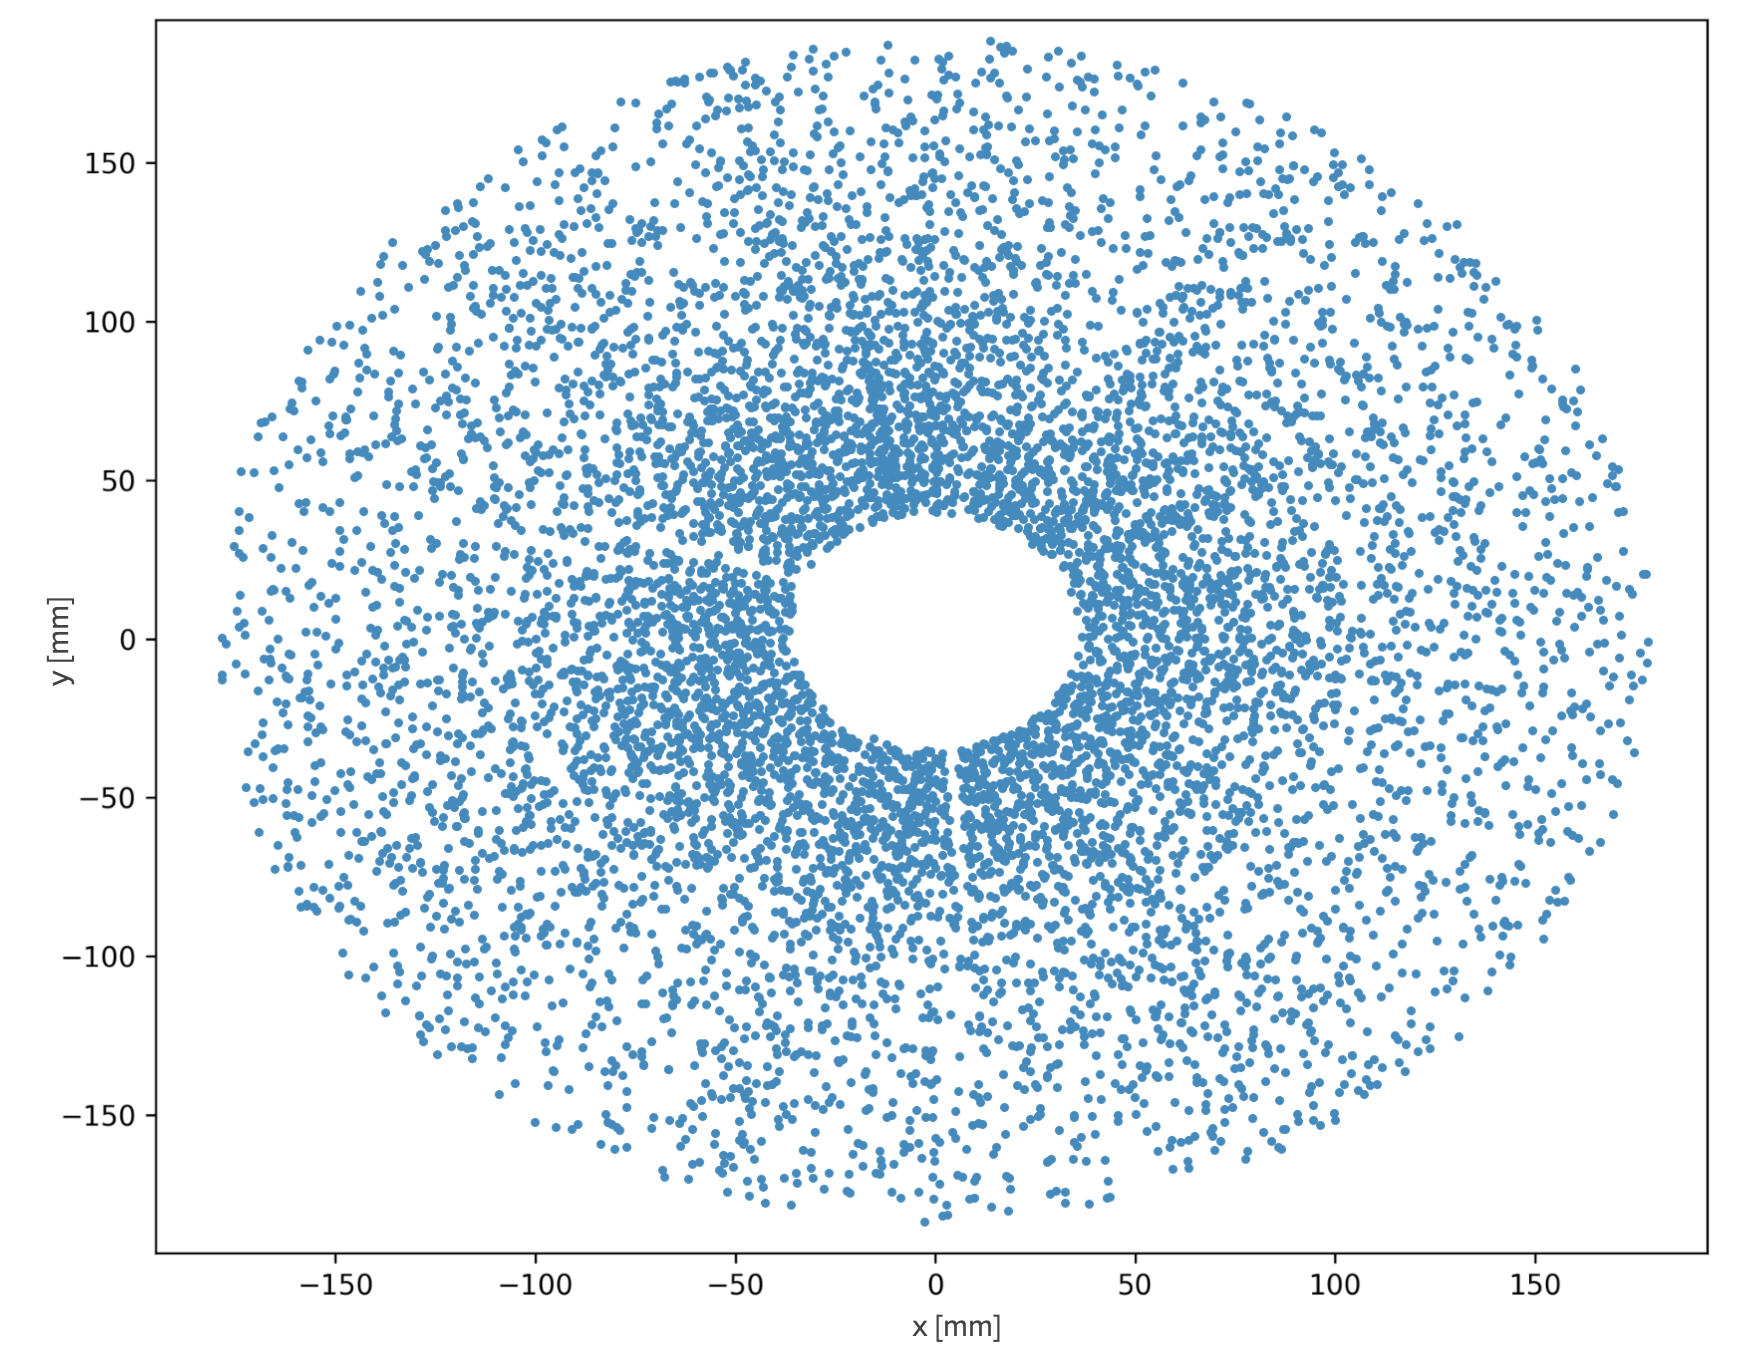
\includegraphics[width=0.51\linewidth]{images/7-results/trackml-endcap-nodes-xy.png}%
        \label{fig:endcap-trackml-sim-xy}%
        }%
    \hfill%
    \subfloat[$r$-$z$ plane view]{%
        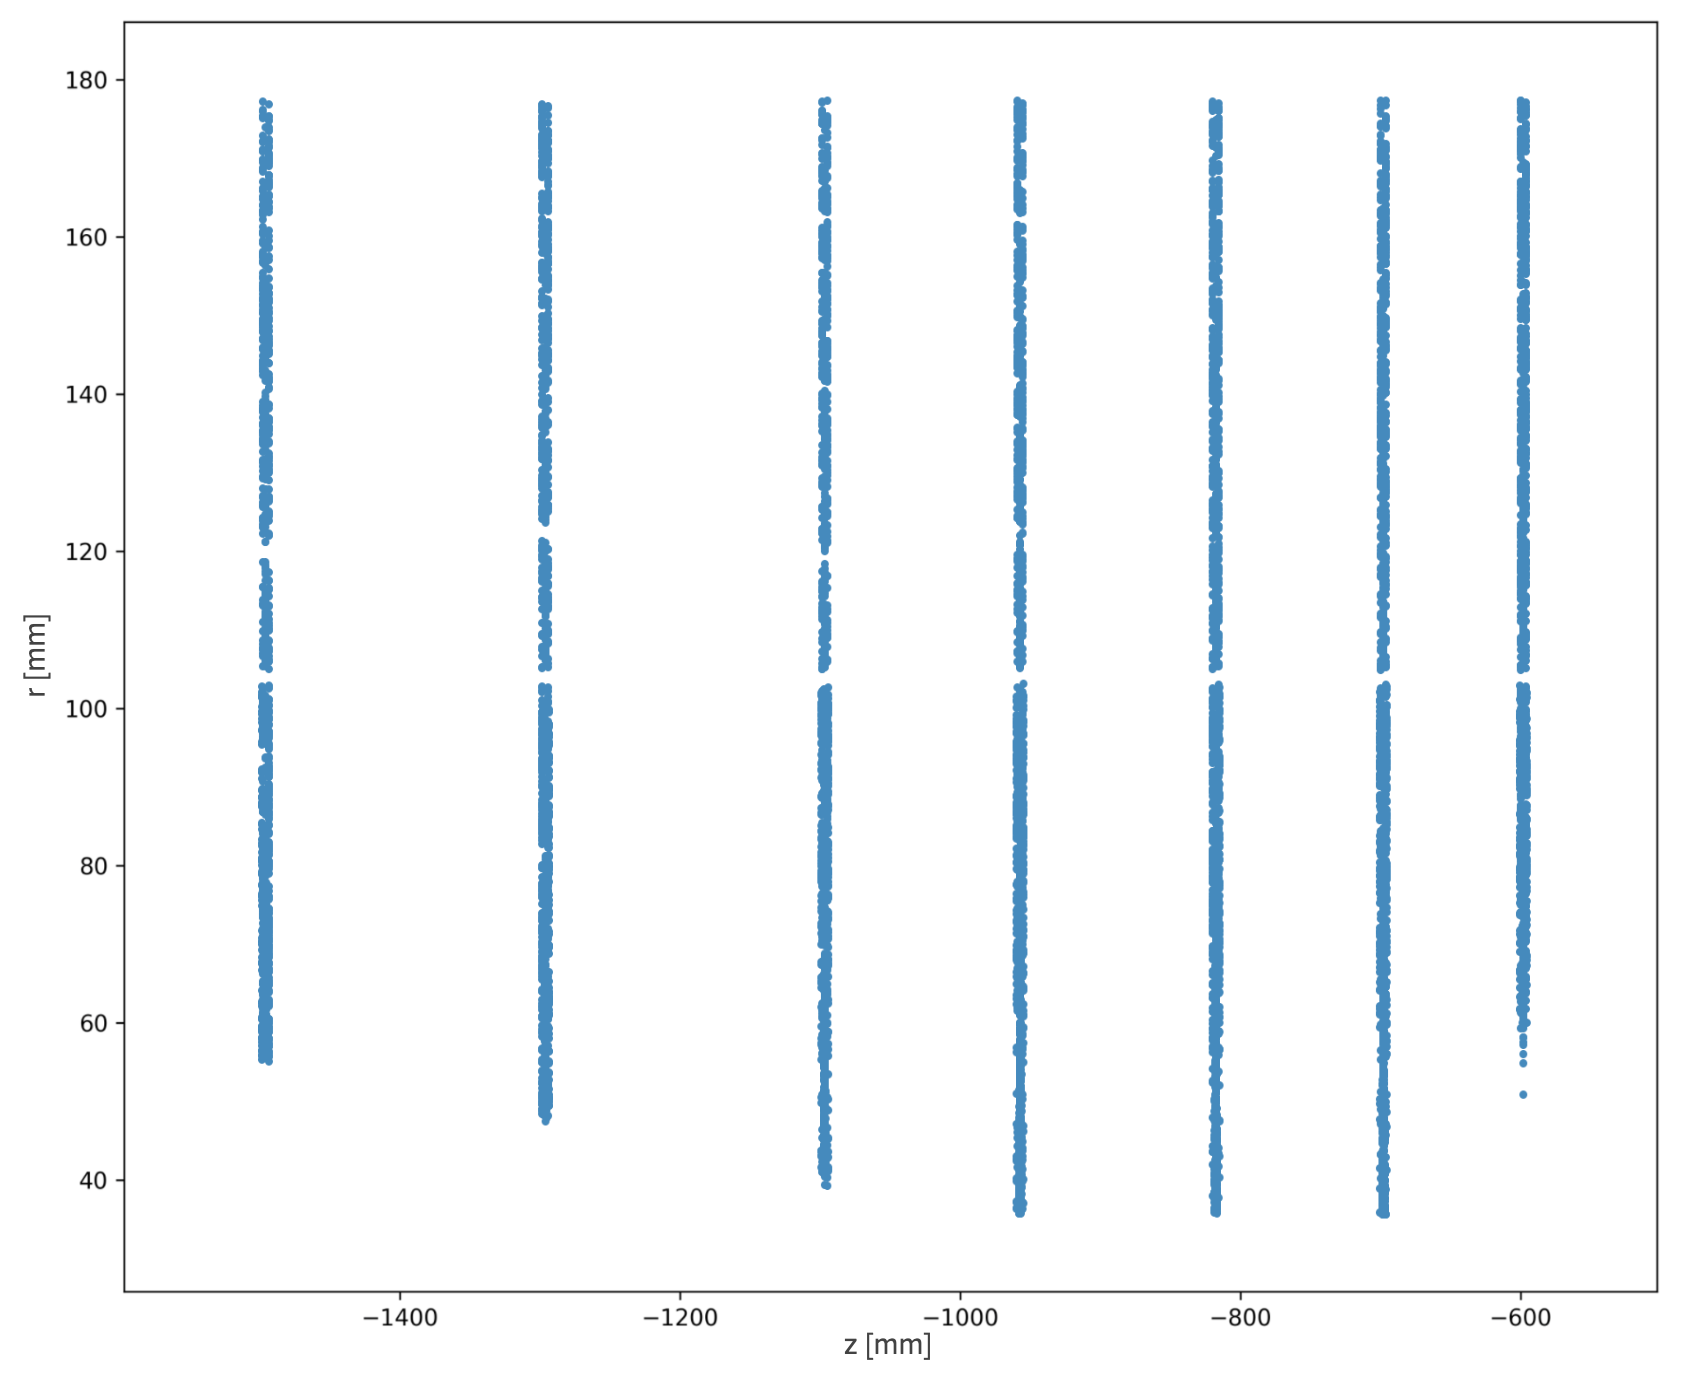
\includegraphics[width=0.49\linewidth]{images/7-results/trackml-endcap-nodes-rz.png}%
        \label{fig:endcap-trackml-sim-rz}%
        }%
    \caption{Event simulation of the TrackML detector isolating volume 7.}
    \label{fig:trackml-results-endcap-nodes-sim}
\end{figure}



\subsection{Performance Evaluation}

The graph network is constructed using 9835 nodes located in volume 7 from a simulated TrackML event and 18,184 predicted edges using the FASTrack algorithm \cite{Dmitry-fasttrack-addtest}, as described in Section \ref{chapter-6-data-prep}. Track state estimates, $X_{ij}$, and edge state covariances, $C_{ij}$, are constructed using the model as described in Section \ref{constructing-track-states}. Figure \ref{fig:trackml-results-endcap-extracted} illustrates the extracted track candidates post Stage 1 of application of the GNN algorithm to volume 7 of the TrackML detector. During this first stage, 960 track candidates were successfully extracted. Figure \ref{fig:trackml-results-endcap-extracted-v2} shows the extracted track candidates post Stage 2 of the GNN algorithm, where a further 265 track candidates were successfully extracted.

\begin{figure}[htbp]%
    \centering
    \subfloat[\centering $x$-$y$ plane view]{{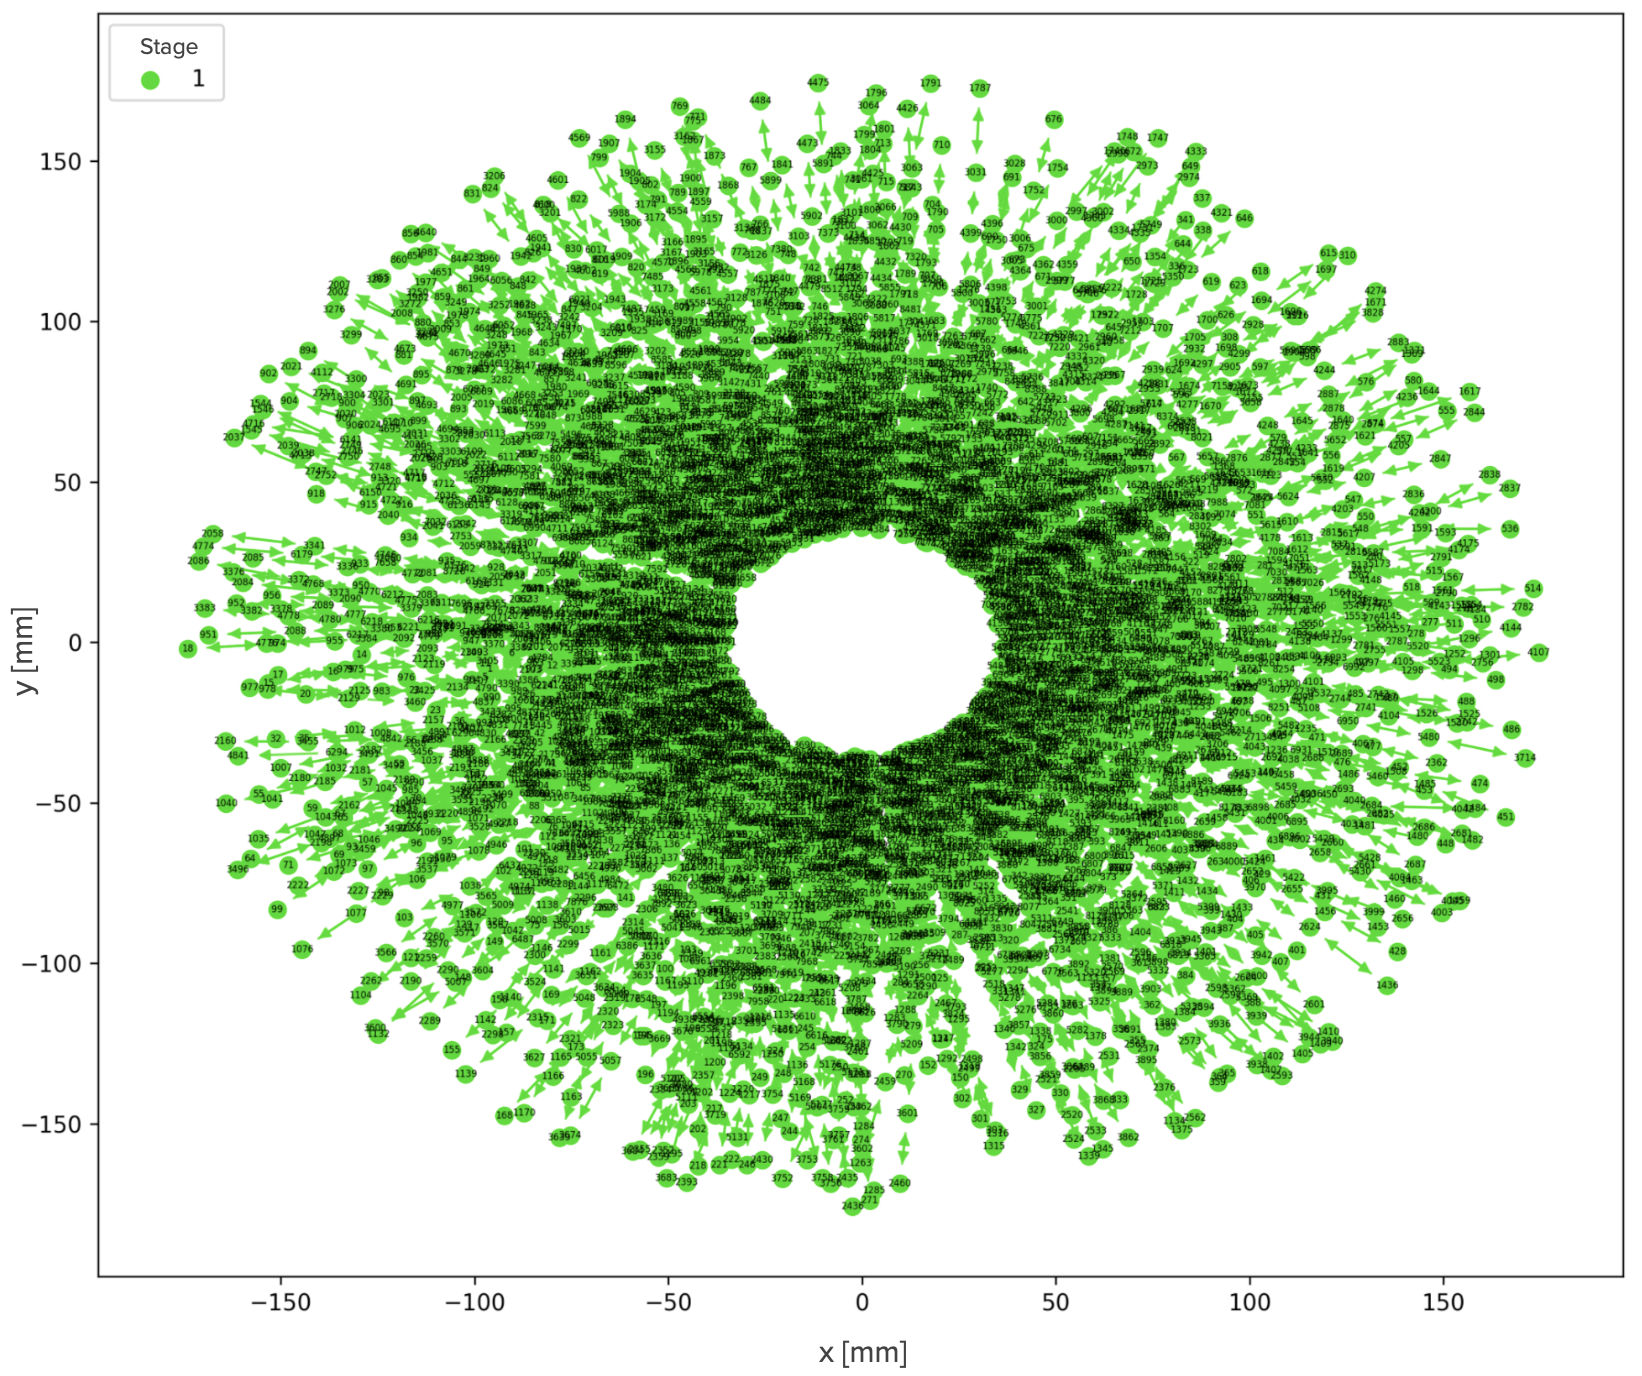
\includegraphics[width=11.5cm]{images/7-results/trackml-endcap-extracted-xy.png} } \label{fig:endcap-trackml-extracted-xy}}%
    \hfill
    %\qquad
    \subfloat[\centering $r$-$z$ plane view]{{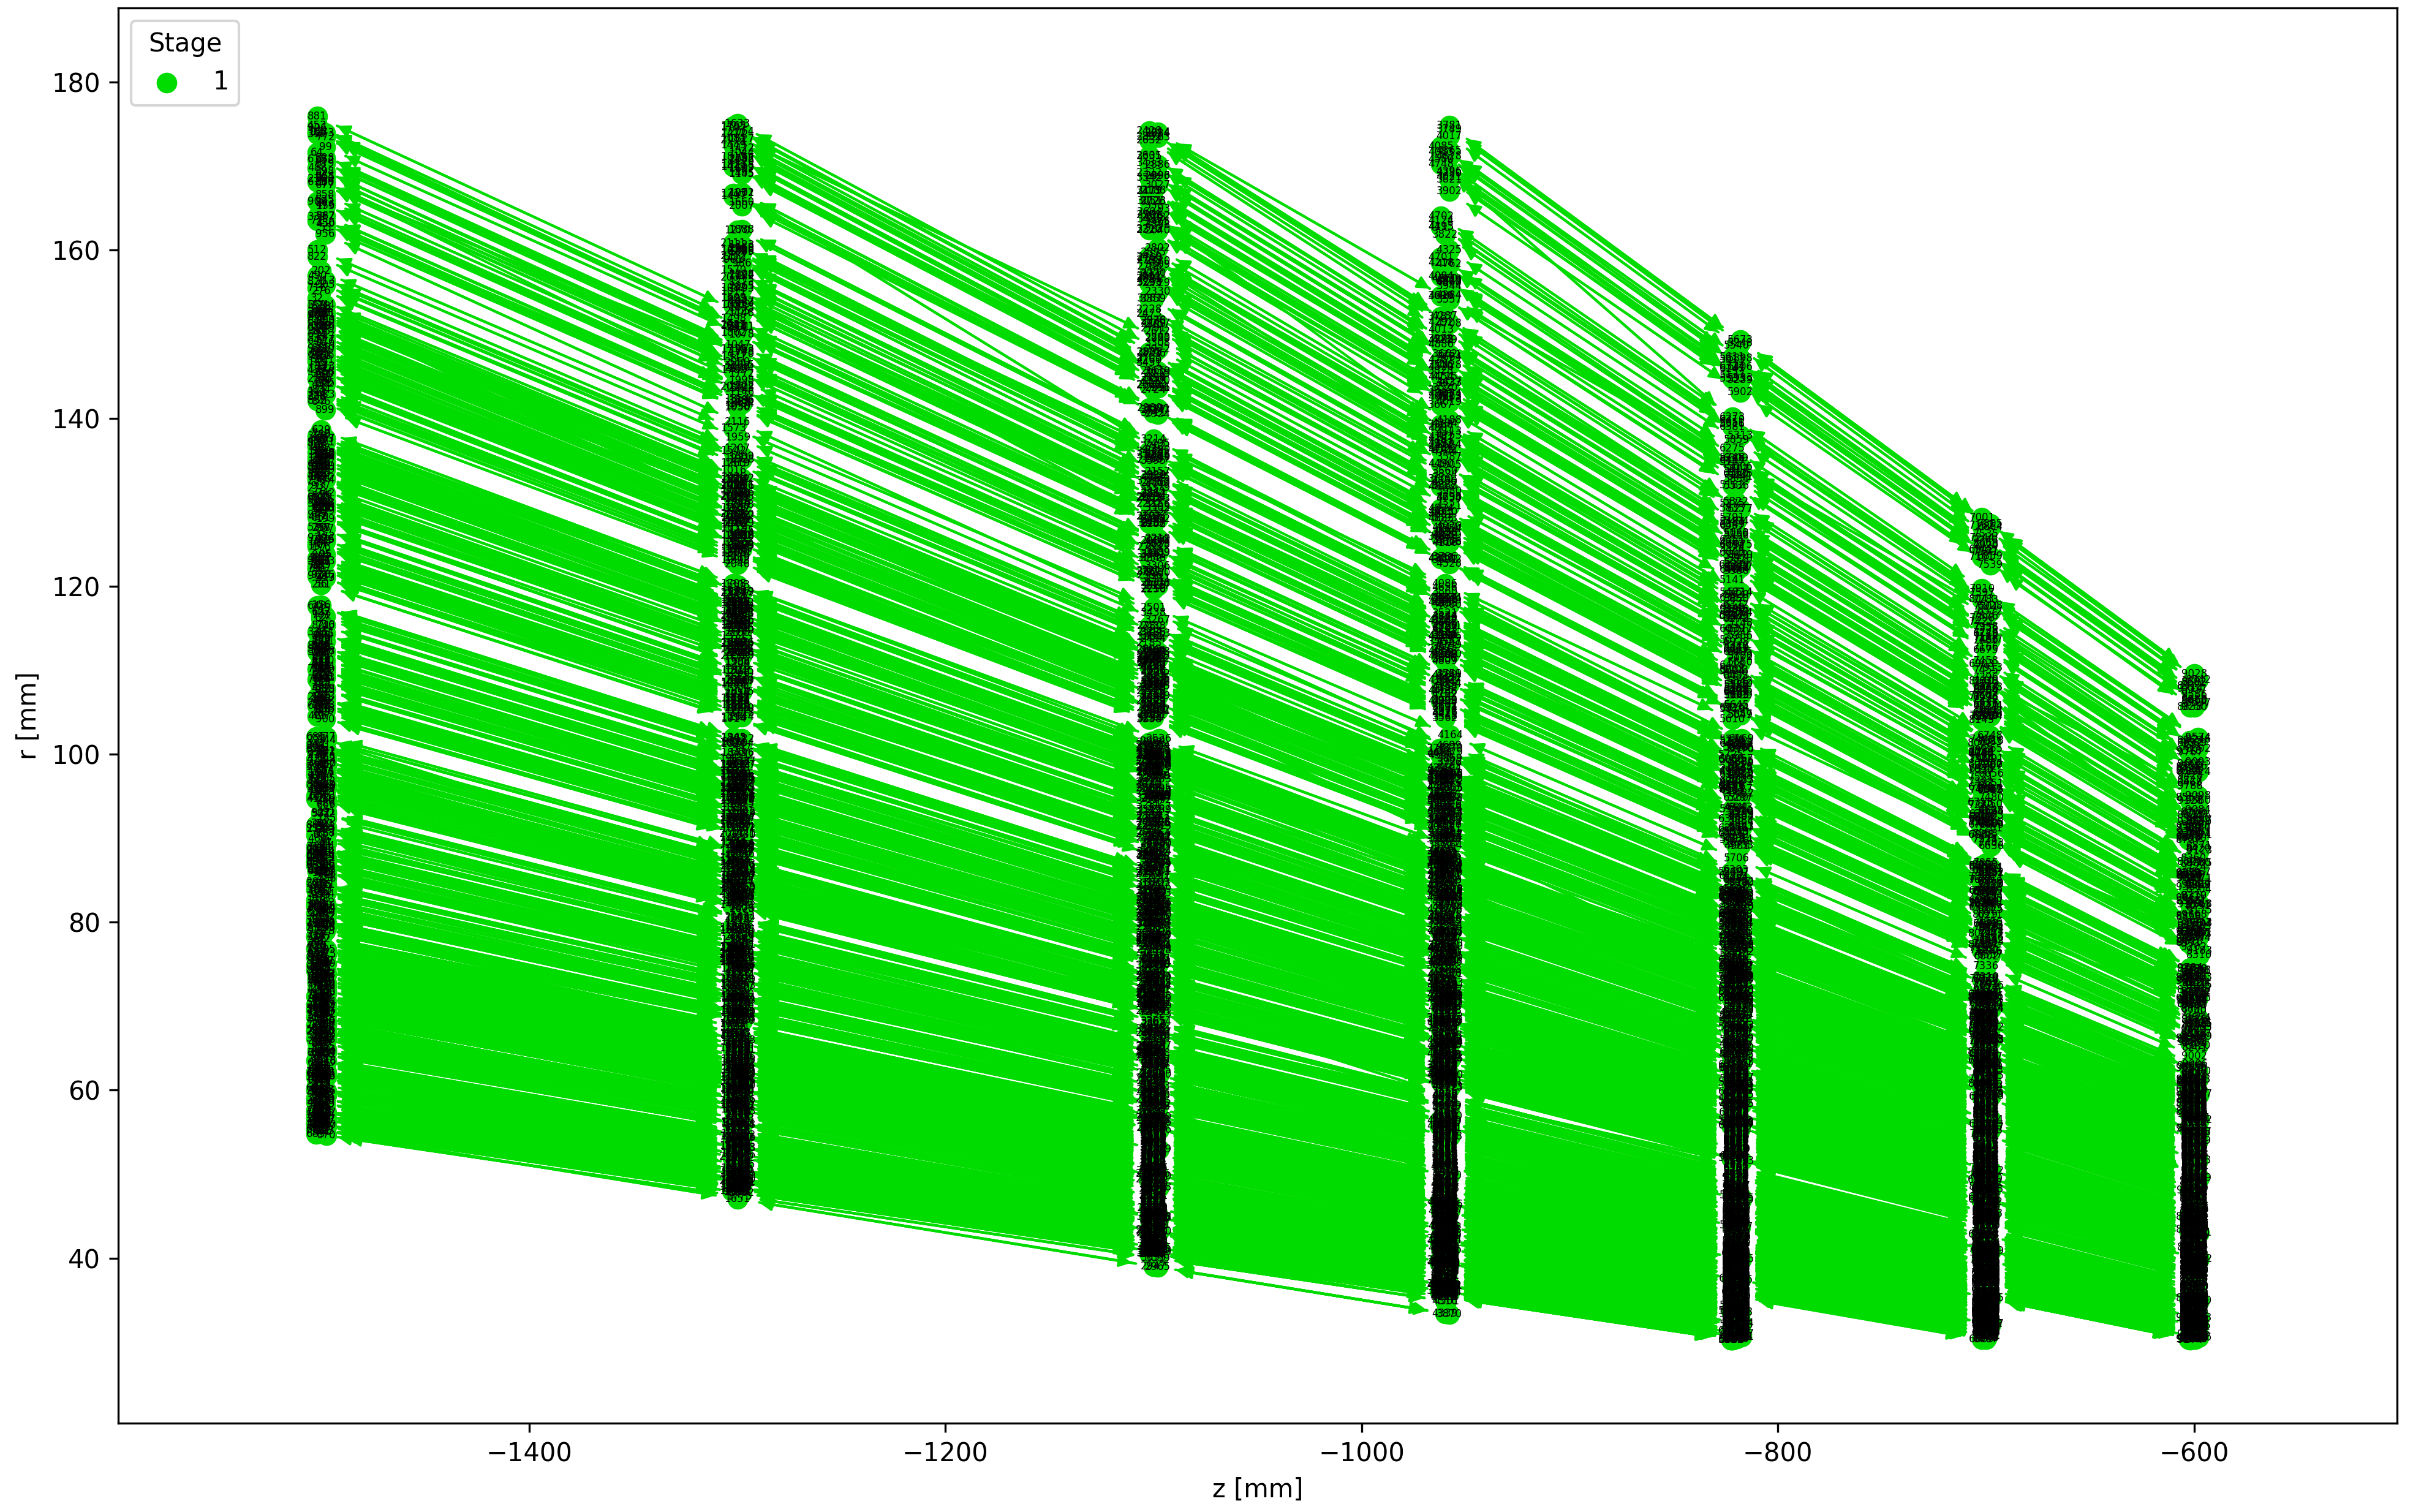
\includegraphics[width=11.5cm]{images/7-results/trackml-endcap-extracted-rz.png} } \label{fig:endcap-trackml-extracted-rz}}%
    \caption{Extracted track candidates post Stage 1 of the GNN algorithm applied to the left Pixel endcap (volume 7) of a simulated TrackML detector event, shown from the view of the a) $x$-$y$ plane and b) $r$-$z$ plane. }%
    \label{fig:trackml-results-endcap-extracted}%
\end{figure}

\begin{figure}[htbp]%
    \centering
    \subfloat[\centering $x$-$y$ plane view]{{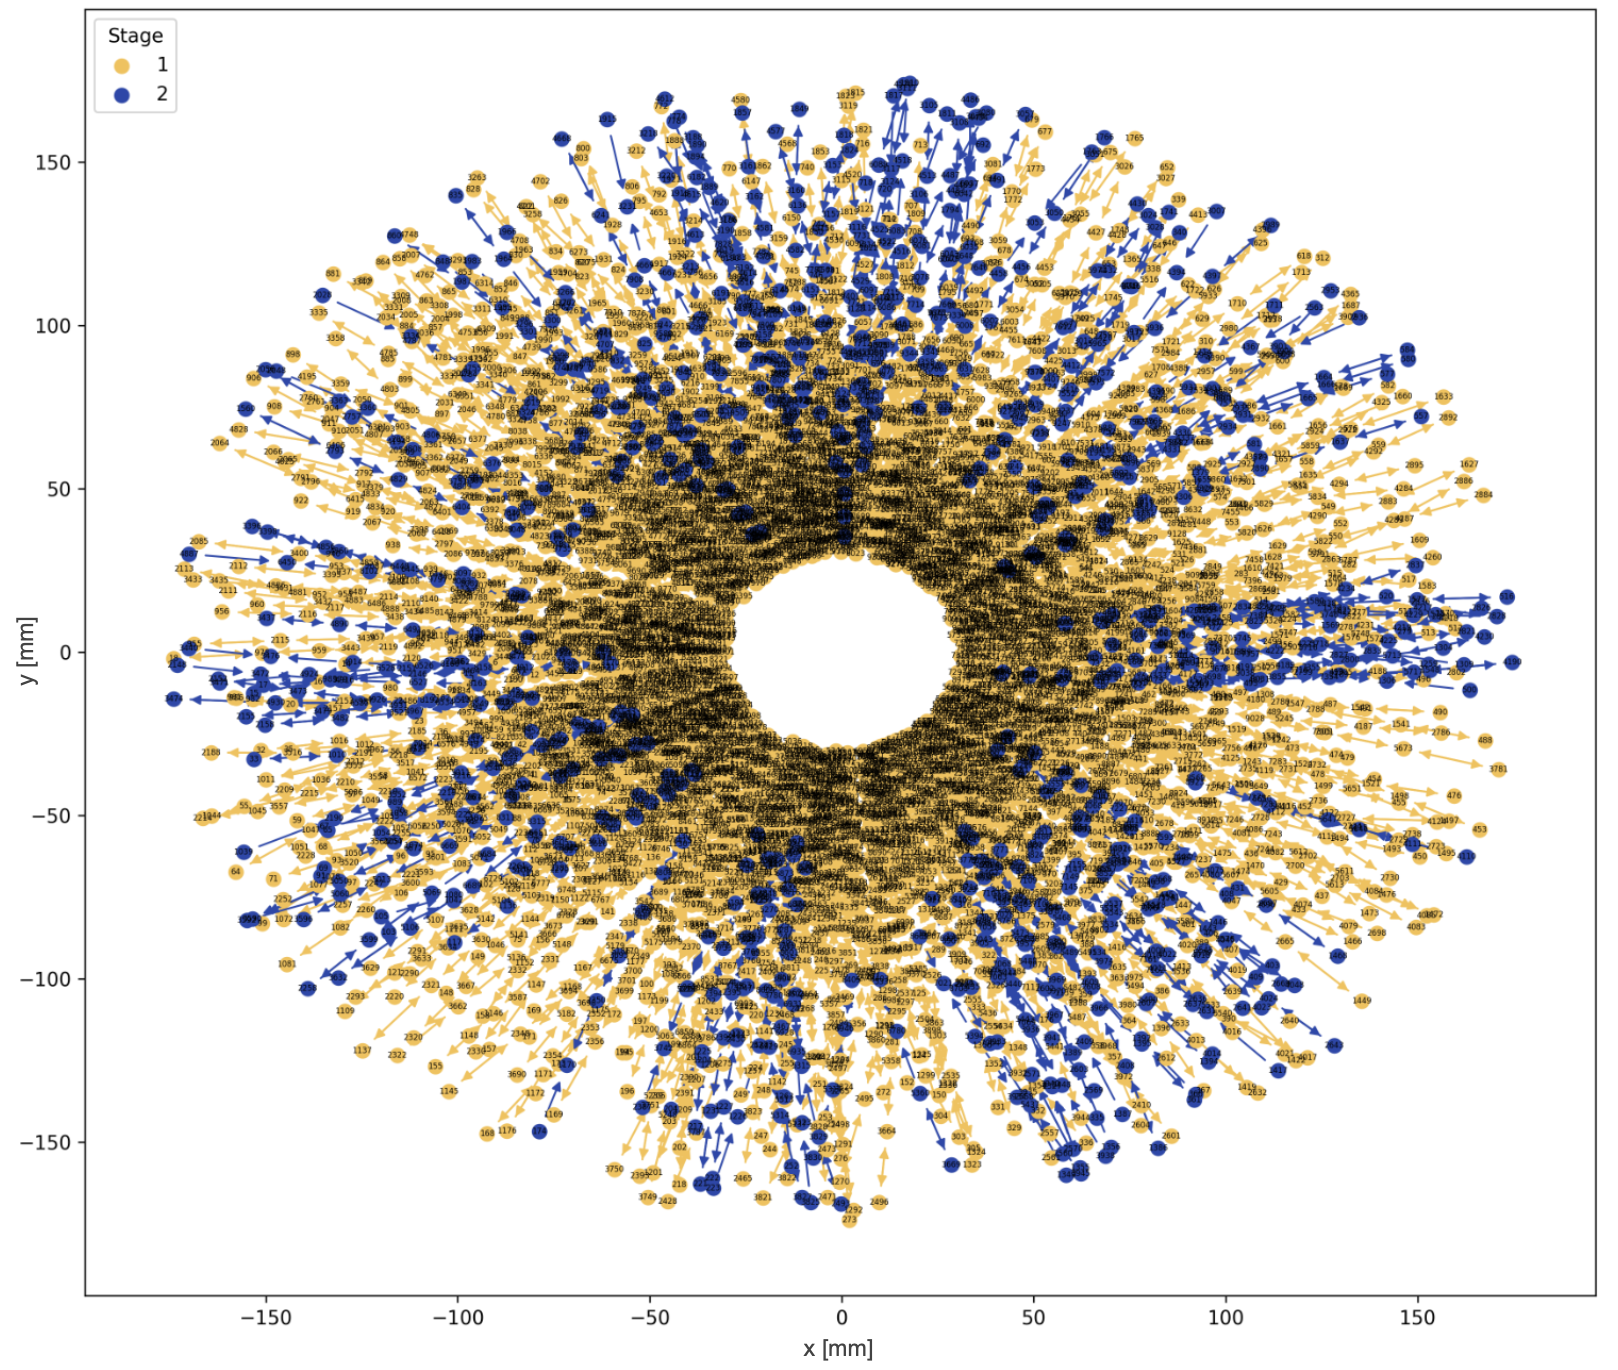
\includegraphics[width=11.5cm]{images/7-results/trackml-endcap-extracted-xy-v2.png} } \label{fig:endcap-trackml-extracted-xy-v2}}%
    \hfill
    %\qquad
    \subfloat[\centering $r$-$z$ plane view]{{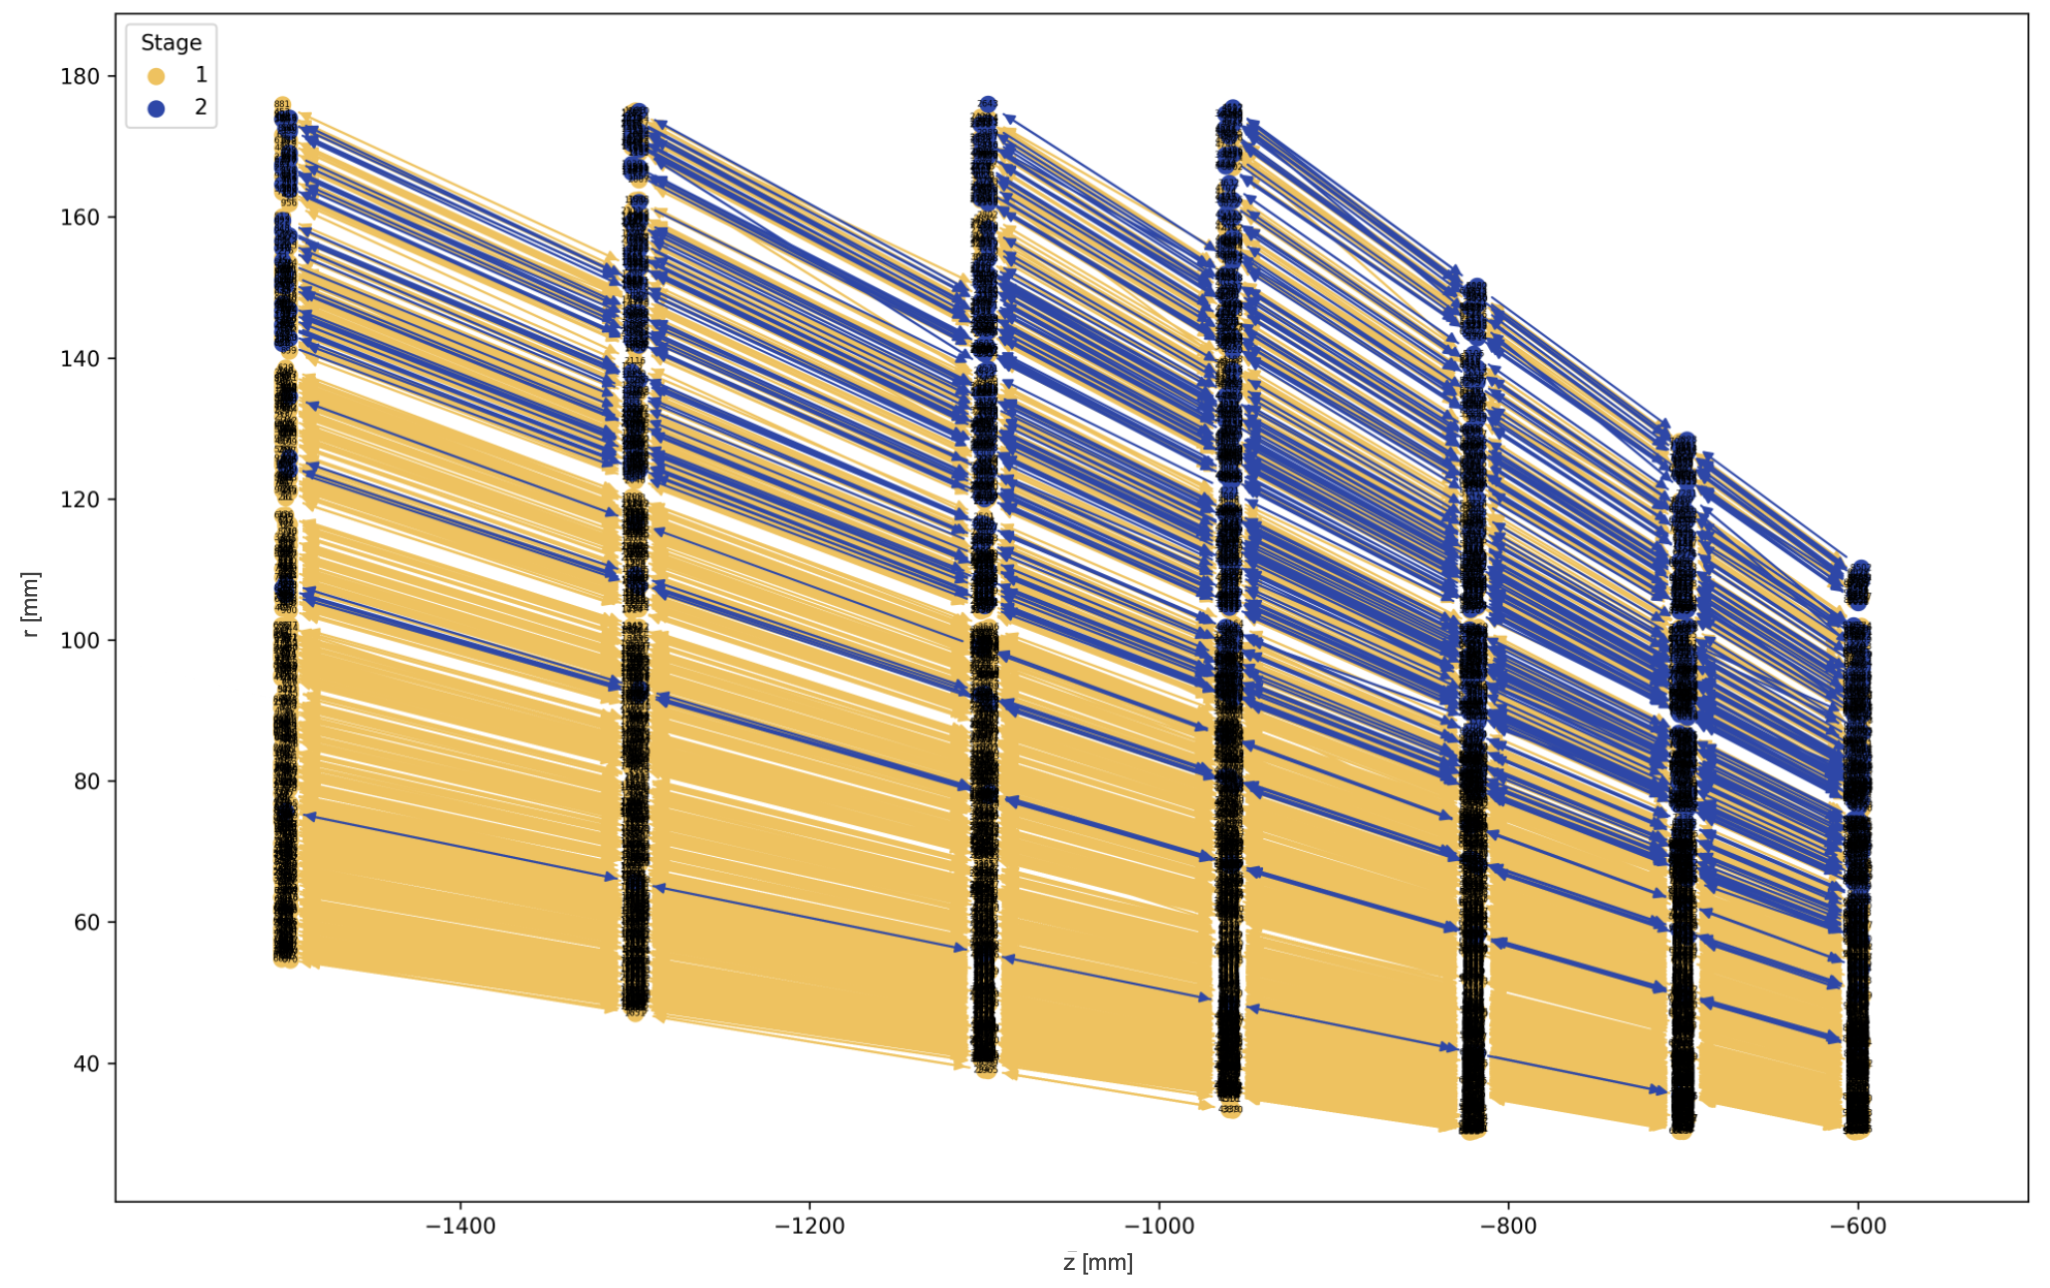
\includegraphics[width=14cm]{images/7-results/trackml-endcap-extracted-rz-v2.png} } \label{fig:endcap-trackml-extracted-rz-v3}}%
    \caption{Extracted track candidates post Stage 1 and 2 of the GNN algorithm applied to the left Pixel endcap (volume 7) of a simulated event of the TrackML detector model, shown from the view of the a) $x$-$y$ plane and b) $r$-$z$ plane.}%
    \label{fig:trackml-results-endcap-extracted-v2}%
\end{figure}

It is clear to see from Figures \ref{fig:endcap-trackml-extracted-xy} and \ref{fig:endcap-trackml-extracted-xy-v2} that track candidates are extracted uniformly within the endcap across all $ 0^{\circ} \leq \phi \leq 360^{\circ}$ during Stage 1 of the GNN algorithm. This is as expected due to the rotational symmetry of the detector in the transverse plane. During Stage 2, we observe the majority of track candidates which are extracted are located at a larger $\theta$ to the $z$-axis (smaller $\eta$). This may be an indication of regions of greater node and edge density, and hence there is a greater proportion of ambiguities to resolve.

The proportion of nodes removed from the main graph network during Stage 1 and Stage 2 were 68\% and 14\% respectively, leaving 18\% of nodes to be further processed. On application of Stage 3 of the GNN algorithm (a further GMR), no additional track candidates were extracted.

% beginning: 9835 nodes
% post stage 1: 3165 nodes
% post stsge 2: 2123 nodes

\subsubsection{Confusion Matrices}
An \textit{outlier edge} is defined to be an edge where its nodes do not belong to the same truth track (truth 1). A \textit{good edge} is defined to be an edge where its nodes do belong to the same truth track (truth 0). The following confusion matrices depict the prediction summary of the GNN algorithm onto the TrackML simulated event, where predicted class 1 indicates the prediction of outlier edges with respect to MC truth and predicted class 0 indicates the prediction of good edges to remain active in the network. The confusion matrix for Stage 1 of the GNN algorithm applied to volume 7 is shown in Figure \ref{fig:confusion-matrix-endcap-stage-1}.

% confusion matrices - endcap stage 1
% Total number of nodes:  9835, edges:  18184
% Total number of nodes with updated states:  9835
% Total number of nodes with a new merged state:  1029
% numerator: 1237 denominator: 1453
% Percentage of correct outliers detected: 85.13420509291122
% true positive number:  1237  false positive number:  216
% true negative number:  2069  false negative number:  136
% Precision: 0.8513420509291122  Recall:  0.9009468317552805
% Normalised confusion matrix
% TPR:  0.9009468317552805  FNR:  0.09905316824471959 
% FPR:  0.09452954048140044  TNR:  0.9054704595185996
\begin{figure}[htbp]%
    \centering
    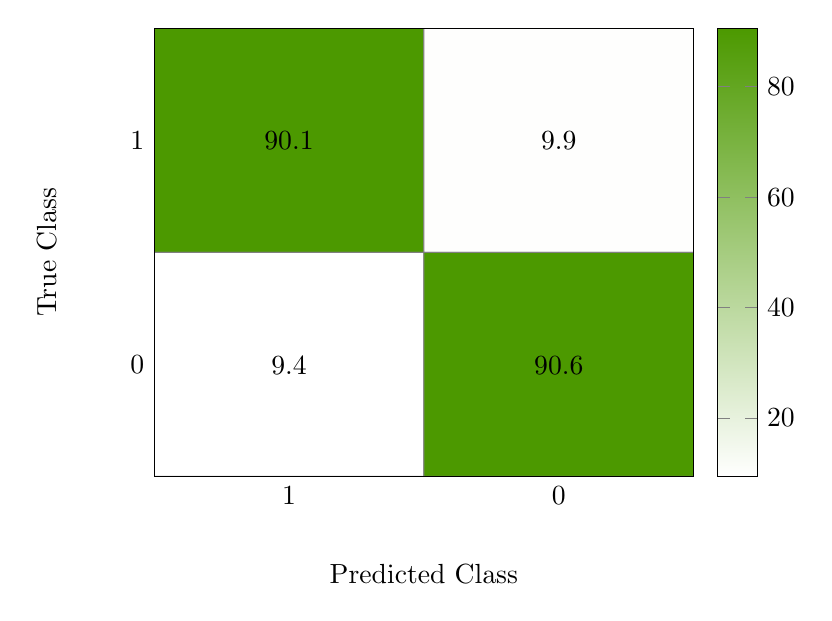
\begin{tikzpicture}
        \begin{axis}[
                colormap={greenyellow}{color=(white) rgb255=(76,153,0)},
                xlabel=Predicted Class,
                xlabel style={yshift=-15pt},
                ylabel=True Class,
                ylabel style={yshift=20pt},
                xticklabels={1, 0}, % changed
                xtick={0,...,1}, % changed
                xtick style={draw=none},
                yticklabels={1, 0}, % changed
                ytick={0,...,1}, % changed
                ytick style={draw=none},
                enlargelimits=false,
                colorbar,
                xticklabel style={rotate=0},
                nodes near coords={\pgfmathprintnumber\pgfplotspointmeta},
                nodes near coords style={yshift=-7pt},
            ]
            \addplot[
                matrix plot,
                mesh/cols=2, % changed
                point meta=explicit,draw=gray
            ] table [meta=C] {
                x y C
                0 0 90.1
                1 0 9.9    
                0 1 9.4
                1 1 90.6
            };
        \end{axis}
    \end{tikzpicture}
    \caption{Confusion matrix percentages for Stage 1 of the GNN algorithm applied to the Pixel endcap (volume 7) of the TrackML detector model.}
    \label{fig:confusion-matrix-endcap-stage-1}
\end{figure}

The TPR for identification of correct outlier edges achieved was 90.1\%, and the True Negative Rate (TNR) in identification of good edges achieved was 90.6\%. With respect to MC ground truth, the proportion of correct outlier edges identified during Stage 1 of the GNN algorithm, and hence the precision, was found to be 85.1\%. The recall in correct outlier edges identified during Stage 1 was 90.1\%. This indicates that the GMR technique of the GNN-algorithm works well for resolving ambiguities in the graph network.

The confusion matrix for Stage 2 of the GNN algorithm applied to volume 7 is shown in Figure \ref{fig:confusion-matrix-endcap-stage-1}.

% confusion matrices - endcap stage 1
% PRINTING ALGORITHM METRICS:
% true positive number:  591  false positive number:  920
% true negative number:  575  false negative number:  162
% Precision: 0.39113170086035737  Recall:  0.7848605577689243
% Normalised confusion matrix
% TPR:  0.7848605577689243  FNR:  0.2151394422310757 
% FPR:  0.6153846153846154  TNR:  0.38461538461538464
\begin{figure}[htbp]%
    \centering
    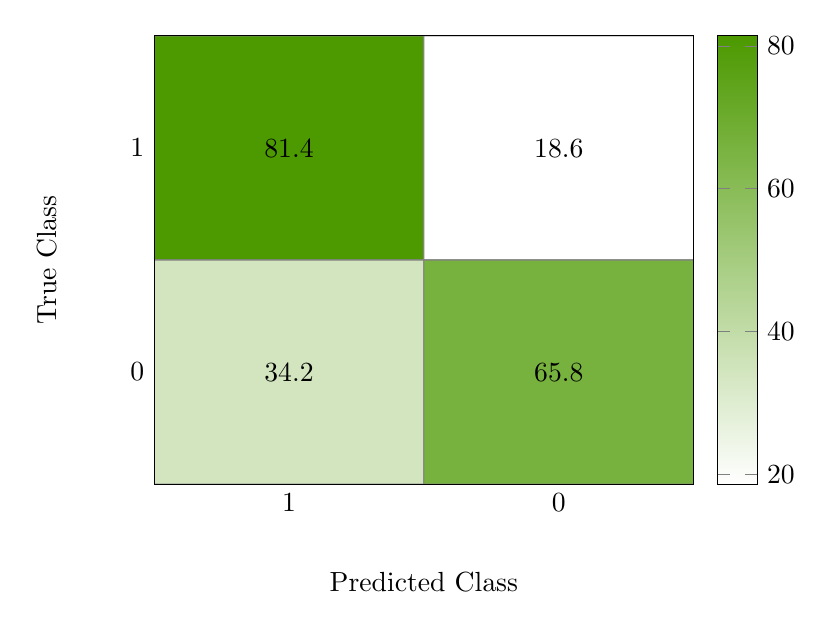
\begin{tikzpicture}
        \begin{axis}[
                colormap={greenyellow}{color=(white) rgb255=(76,153,0)},
                xlabel=Predicted Class,
                xlabel style={yshift=-15pt},
                ylabel=True Class,
                ylabel style={yshift=20pt},
                xticklabels={1, 0}, % changed
                xtick={0,...,1}, % changed
                xtick style={draw=none},
                yticklabels={1, 0}, % changed
                ytick={0,...,1}, % changed
                ytick style={draw=none},
                enlargelimits=false,
                colorbar,
                xticklabel style={rotate=0},
                nodes near coords={\pgfmathprintnumber\pgfplotspointmeta},
                nodes near coords style={yshift=-7pt},
            ]
            \addplot[
                matrix plot,
                mesh/cols=2, % changed
                point meta=explicit,draw=gray
            ] table [meta=C] {
                x y C
                0 0 81.4
                1 0 18.6     
                0 1 34.2
                1 1 65.8
            };
        \end{axis}
    \end{tikzpicture}
    \caption{Confusion matrix percentages for Stage 2 of the GNN algorithm applied to the Pixel endcap (volume 7) of the TrackML detector model.}
    \label{fig:confusion-matrix-endcap-stage-2}
\end{figure}

For Stage 2, the TPR for identification of correct outlier edges, and hence the recall, achieved was 81.4\%, and the TNR in identification of good edges achieved was 65.8\%. With respect to MC ground truth, the precision in correct outlier edges identified during Stage 2 was found to be 69.8\%. In comparison to the prediction summary for Stage 1 shown in Figure \ref{fig:confusion-matrix-endcap-stage-1}, the second stage of the GNN algorithm does not discriminate between both classes as well as Stage 1. During Stage 2, we observe an increase in the prediction of false positives. This indicates that the algorithm begins to falsely predict a greater proportion of outlier edges, which will then affect the network connections in further algorithm stages.






\subsubsection{Track Reconstruction Efficiency and Purity Metrics}

The track reconstruction efficiency, $\epsilon$, provides an indication of the performance of the algorithm and is defined as the ratio of successfully reconstructed reference tracks, $n_R$, to the total number of reconstructable reference tracks, $N_R$, in a given volume of interest and is given by Eq \eqref{eqn:reoncstruction-eff}. 


\begin{equation}
    \epsilon = \frac{n_R}{N_R}
    \label{eqn:reoncstruction-eff}
\end{equation}

A reconstructable reference track is defined as a fully connected track within the volume of interest. As the TrackML detector can produce up to 4 hits per detector layer, ...


We require at least 11 hits within the region of interest to be considered as a reconstructable reference track...

Successfully reconstructed reference tracks is defined as having at least 50\% of its hits from the same truth particle $N_{hits}$. If ...

% TODO: put the following information in a table?
For fully contained MC truth tracks within volume 7 of the TrackML Pixel detector with $p_{T} \geq$ 150MeV, the track reconstruction efficiency obtained was 86.2\%, where $n_R = 614$ and $N_R = 712$. Similarly, for fully contained MC truth tracks within volume 7 of the TrackML Pixel detector with $p_{T} \geq$ 1GMeV the track reconstruction efficiency obtained was 93.8\%, where $n_R = 180$ and $N_R = 192$.


% \begin{table}[!htbp]
% \caption{.....}
% \begin{center}
% \begin{tabular}{cccc}
% \toprule
% $p_{\text{T}}$ & $n_R$ & $N_R$ & $\epsilon$ (\%) \\
% \hline
% $\geq$ 150MeV & 614 & 712 & 86.2 \\
% $\geq$ 1GeV & 180 & 192 & 93.8\\
% \bottomrule
% \end{tabular}
% \end{center}
% \label{tab:track-reconstruction-eff-gnn-results}
% \end{table}




%For fully contained MC truth tracks within volume 7 of the TrackML Pixel detector with $p_{T} \geq$ 150MeV, the track reconstruction efficiency obtained was 86.2\%, where the $n_R$ = 614 and $N_R$ = 712, and for $p_{T} \geq$ 1GMeV the track reconstruction efficiency obtained was 93.8\%, where the $n_R$ = 183 and $N_R$ = 195.


% Total num of reconstructed tracks: 180
% Total num of reference tracks: 192
% Track reconstruction efficiency:  93.750 %


%Particles with four or more hits contained within volume 7 are considered and only proposed tracks with four or more hits are considered. Each track is matched with the ground truth majority particle sharing with it the greatest hit number $N_{truth}$. The ratio of $N_{truth}$ to the number of hits $N_{hits}$ for the reconstructed track defines the track purity, whilst the ratio of this to the number of hits of the underlying particle defines the particle purity. Both the track purity and particle purity must be $>$ 50\%. This criteria coincides with the definition of an accepted track candidate stated in the TrackML competition \cite{trackml}. The resulting average track purity and particle purity for all extracted candidates in volume 7 after Stages 1 and 2 of application of the GNN algorithm is 99\%. The purity distributions shown in Figure \ref{fig:purity} indicate that the application of the OU process works well for the given $p_{T}$ range.


\begin{figure}[htbp]
    \centering
    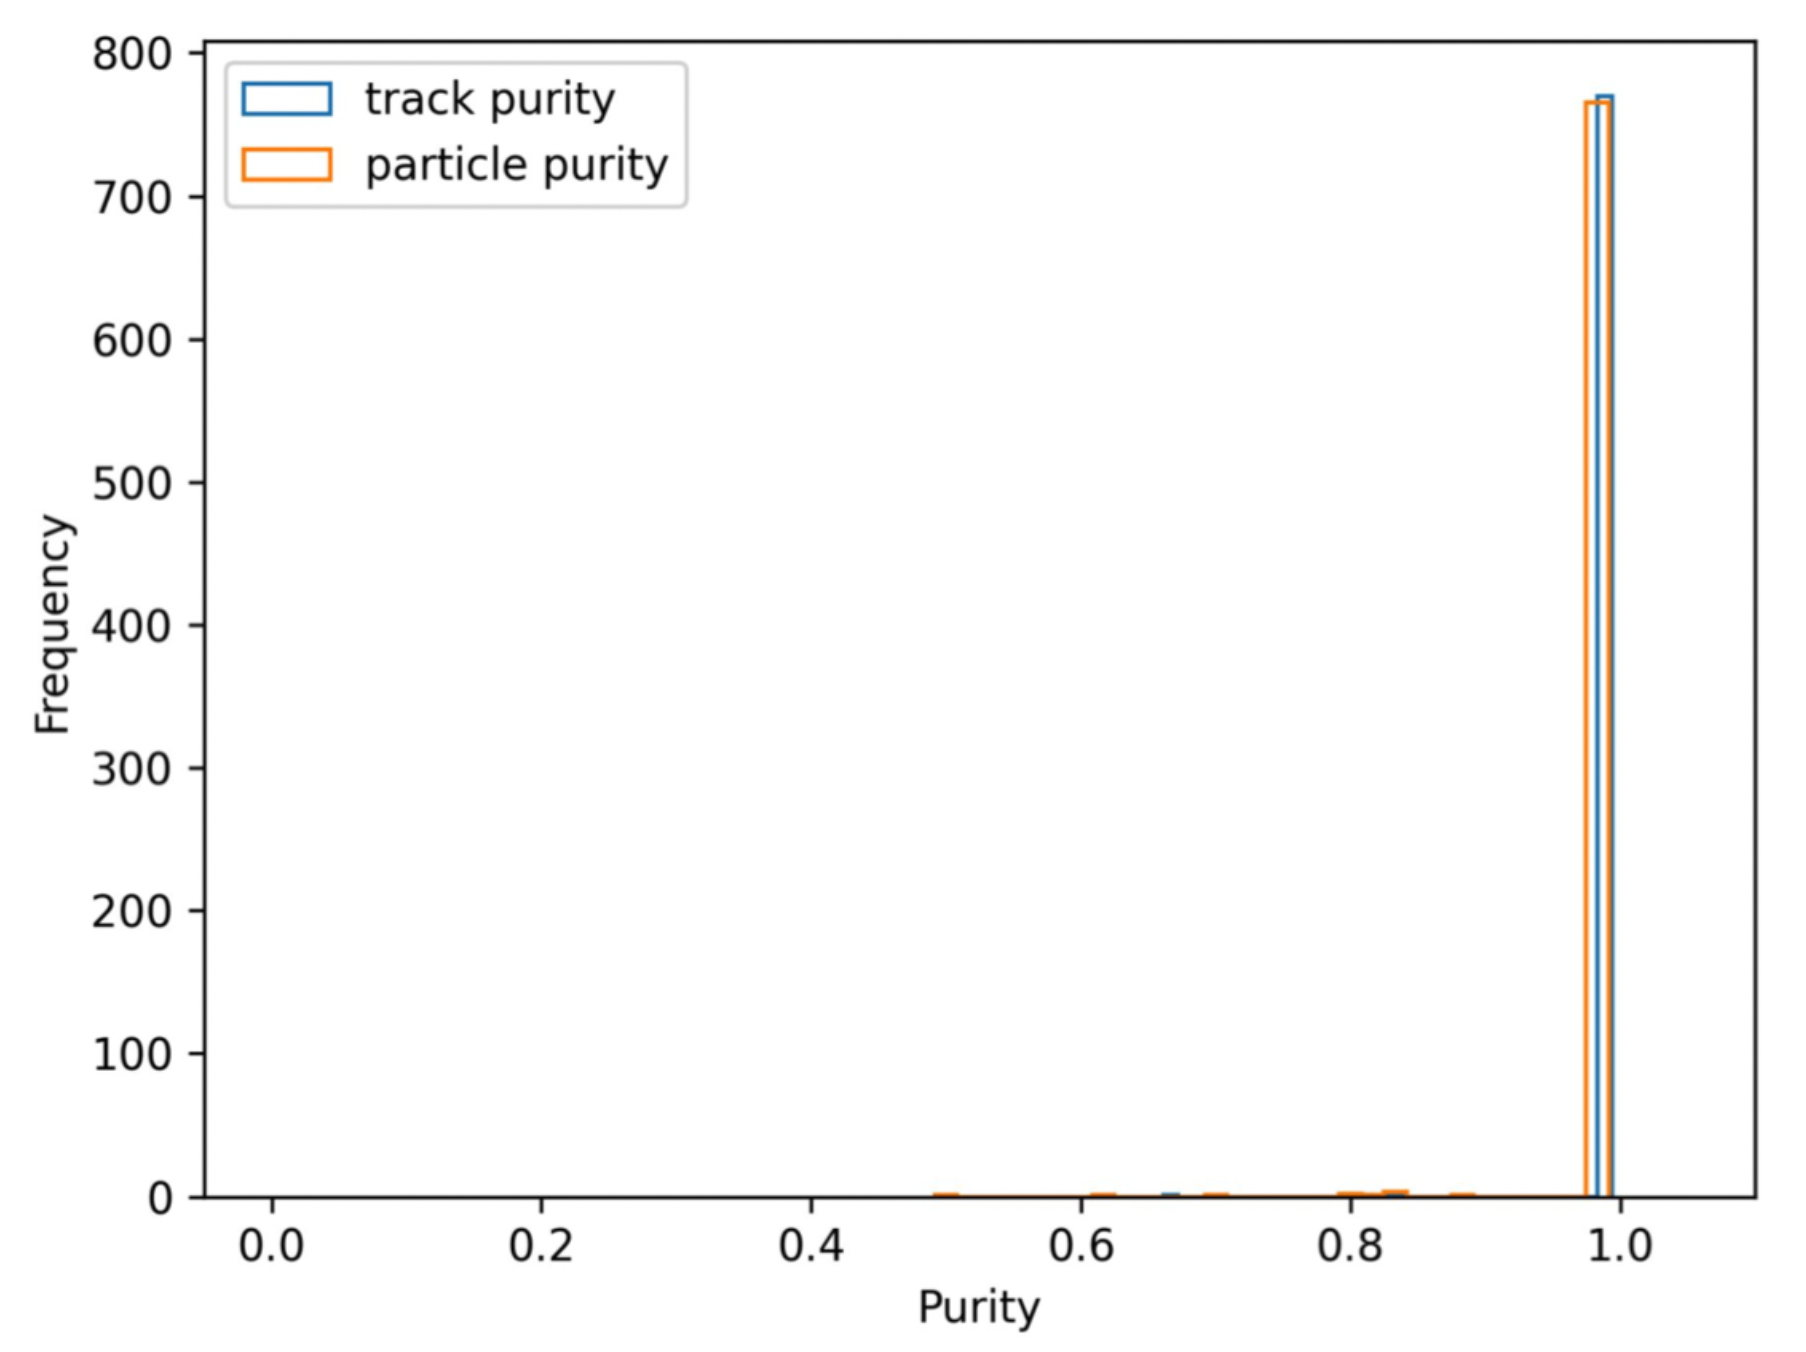
\includegraphics[width=0.7\textwidth]{images/7-results/endcap-purity.png}
    \caption{Purity distributions for application of the GNN algorithm for track reconstruction on the left Pixel endcap (volume 7) of the TrackML detector}
    \label{fig:trackml-results-endcap-nodes-purity}%
\end{figure}

%present the average over many events here
Executing the GNN algorithm on volume 7 of the TrackML detector and averaging over 70 simulated events, the average track reconstruction efficiency achieved was .... The average track purity and average particle purity achieved were both 99\%.



\subsubsection{Execution Times}

The GNN algorithm was executed on a MacOS machine, M1 Pro chip, 16GB RAM, with no multi-threaded functions. The minimum execution time for the GNN algorithm to process 1 simulated event in volume 7 of the TrackML detector was 45.6s. Figure \ref{fig:execution-time-endcap-1} shows a breakdown in execution time for each stage of the GNN algorithm.

\begin{figure}[htbp]
    \centering
    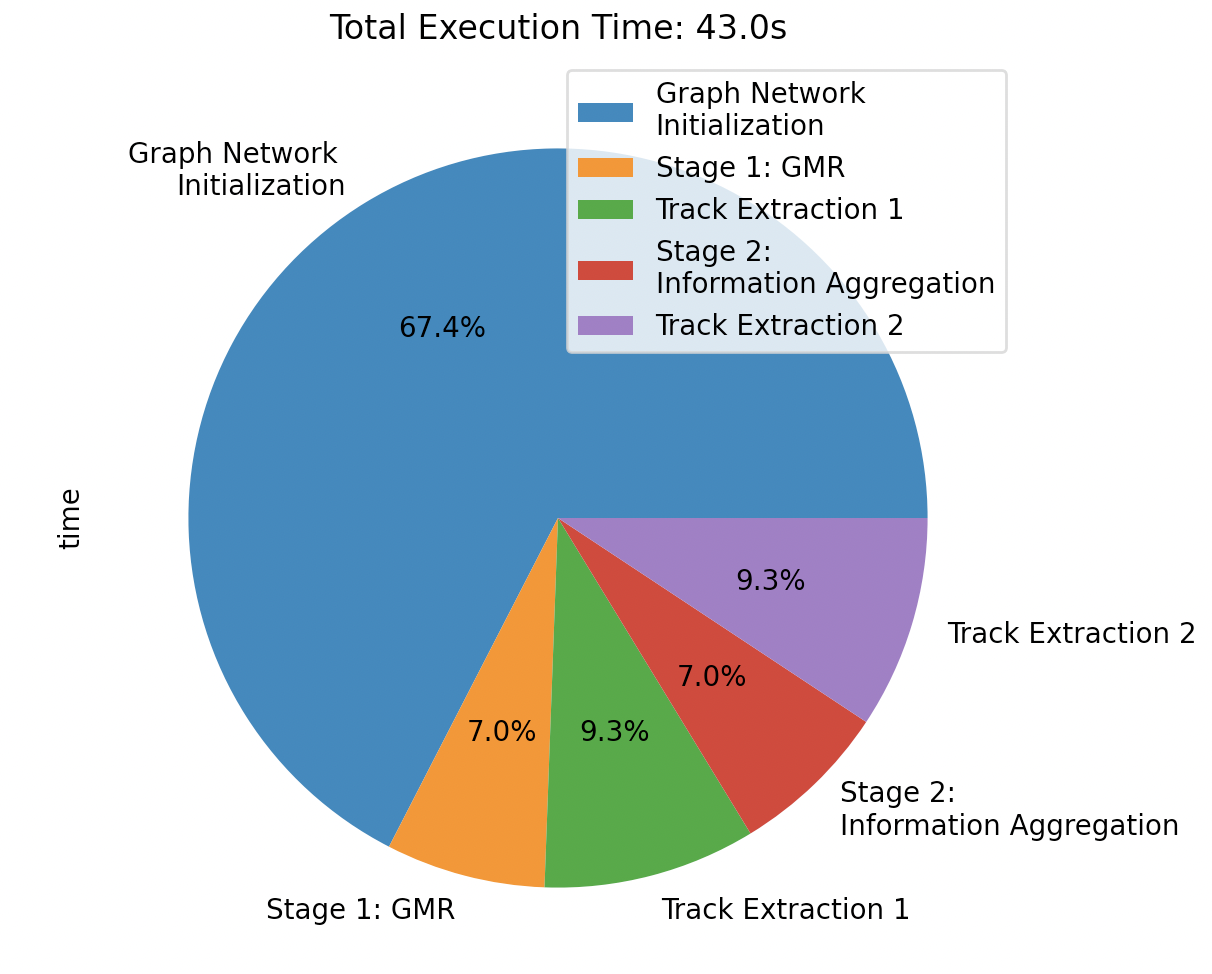
\includegraphics[width=0.7\textwidth]{images/7-results/execution-time-endcap-1.png}
    \caption{Breakdown of execution time for each stage of the GNN algorithm applied to volume 7 of the TrackML detector.}
    \label{fig:execution-time-endcap-1}%
\end{figure}


The initialization of the graph network adopts the majority of the execution time, where the remaining algorithmic components comprise 15.9s in execution time. Graph network initialization comprises of a conversion of TrackML hit data to nodes and edges, as well as construction of track state estimates $X_{ij}$ and covariances $C_{ij}$. Reading and writing into the graph network implemented using the NetworkX library ....

% TODO: comparison with other algorithms??


% \begin{figure}[htbp]
%     \centering
%     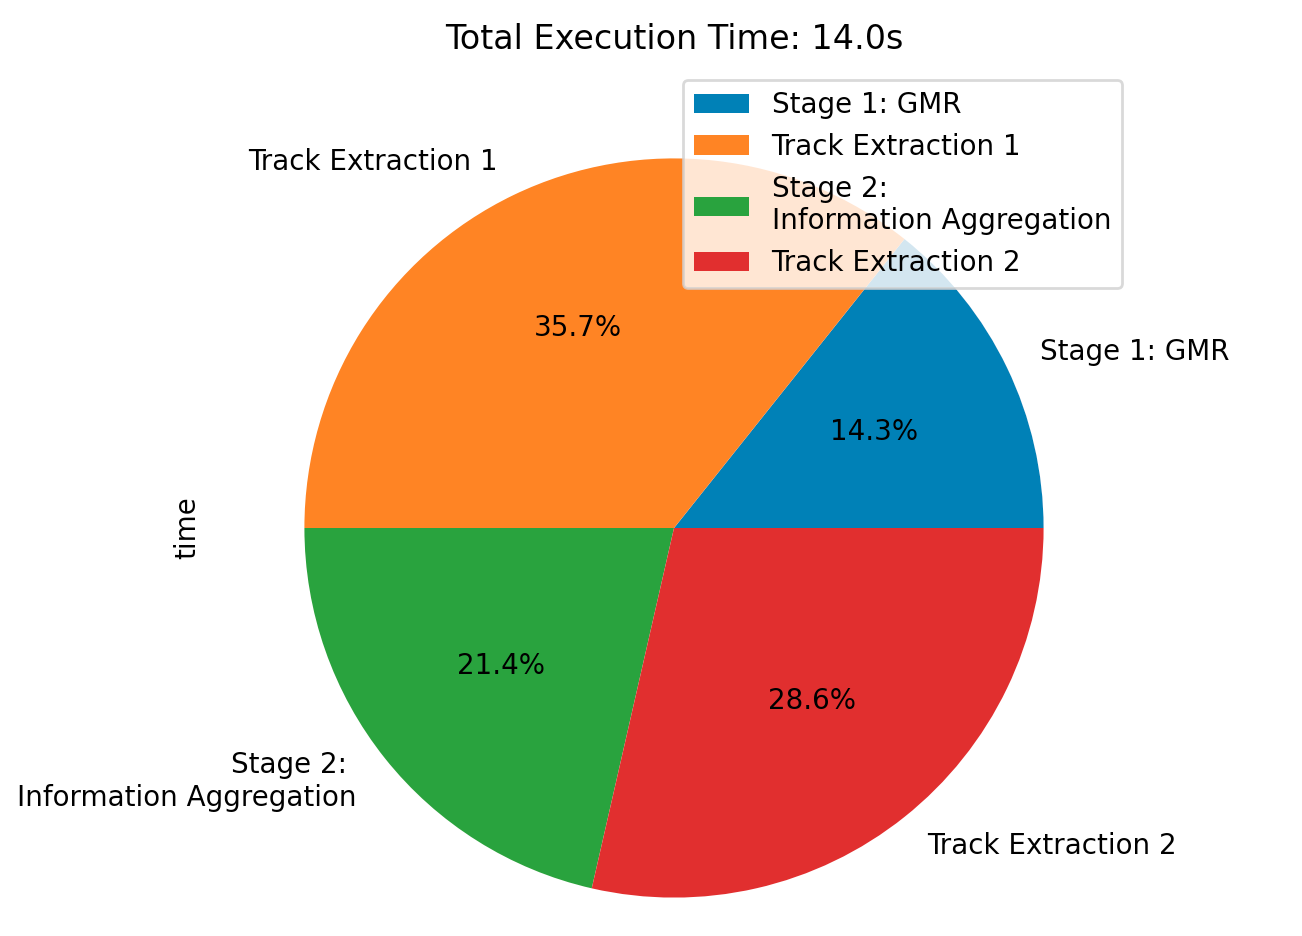
\includegraphics[width=0.7\textwidth]{images/7-results/execution-time-endcap-2.png}
%     \caption{Breakdown of execution time for each stage of the GNN algorithm applied to volume 7 of the TrackML detector, excluding network initialization.}
%     \label{fig:execution-time-endcap-2}%
% \end{figure}




\subsubsection{Advantages of the KF Application}

An important feature of the application of the KF is that reconstruction of curved tracks is possible using a low-dimensionality model. By assuming a slow change in track direction, a special dynamic model for the KF is constructed using the OU process. The OU process implicitly takes into account the track curvature, without the need to extend the track state to contain additional parameters.








\section{Outlook and Further Work}
\label{chapter-7-outlook}

\subsection{Extension to the Pixel Barrel Region}

The application of the GNN algorithm is extended to the Pixel barrel region and the right endcap of the TrackML detector, in order to cover the entire Pixel detector volumes $\{7, 8, 9\}$, with reference to Figure \ref{fig:trackml-detector-image}. The graph network is constructed using 38,365 nodes contained within these volumes from a simulated TrackML event, and 201,748 predicted edges are formed using the FASTrack algorithm \cite{Dmitry-fasttrack-addtest}. Figure \ref{fig:trackml-results-barrel-endcap} illustrates the extracted track candidates after application of the GNN algorithm. 

It is clear to see from Figure \ref{fig:trackml-results-barrel-endcap-extracted-xy} that track candidates are extracted uniformly across all $ 0^{\circ} \leq \phi \leq 360^{\circ}$ during Stages 1 and 2 of the GNN algorithm. This is as expected due to the rotational symmetry of the detector in the transverse plane. 

Figure \ref{fig:trackml-results-barrel-endcap-extracted-rz} shows the extracted track candidates viewed from the $r$-$z$ plane, where the algorithm works effectively in both the left and right Pixel endcap regions, however the proportion of track candidates extracted in the Pixel barrel is significantly less. During the Stage 1, a total of 1629 track candidates were successfully extracted. During Stage 2 a further 294 track candidates were extracted and in Stage 3 a further 7 were extracted.

In Stage 1, we observe track candidates to be extracted uniformly throughout both endcaps. This is primarily due to the parallel geometry of detector layers and hence telescopic trajectory of the corresponding tracks. This means there are far fewer ambiguities to resolve in comparison to the barrel region. In contrast to this, during Stage 2 we observe the majority of track candidates extracted to be located at a larger $\theta$ to the $z$-axis (smaller $\eta$) in comparison to Stage 1. This is the transition region between the barrel and endcap layers. We also observe a small proportion of track candidates extracted which are contained only within the barrel region.

A greater proportion of track candidates located at .... the transition between the barrel and endcap layers ...are ex The node density in the barrel is ... times greater compared to the endcap regions, and the edge density is .... which is a contributing factor towards this.



%Comment on the proportion of nodes removed at each stage


\begin{figure}[htbp]%
    \centering
    \subfloat[\centering $x$-$y$ plane view]{{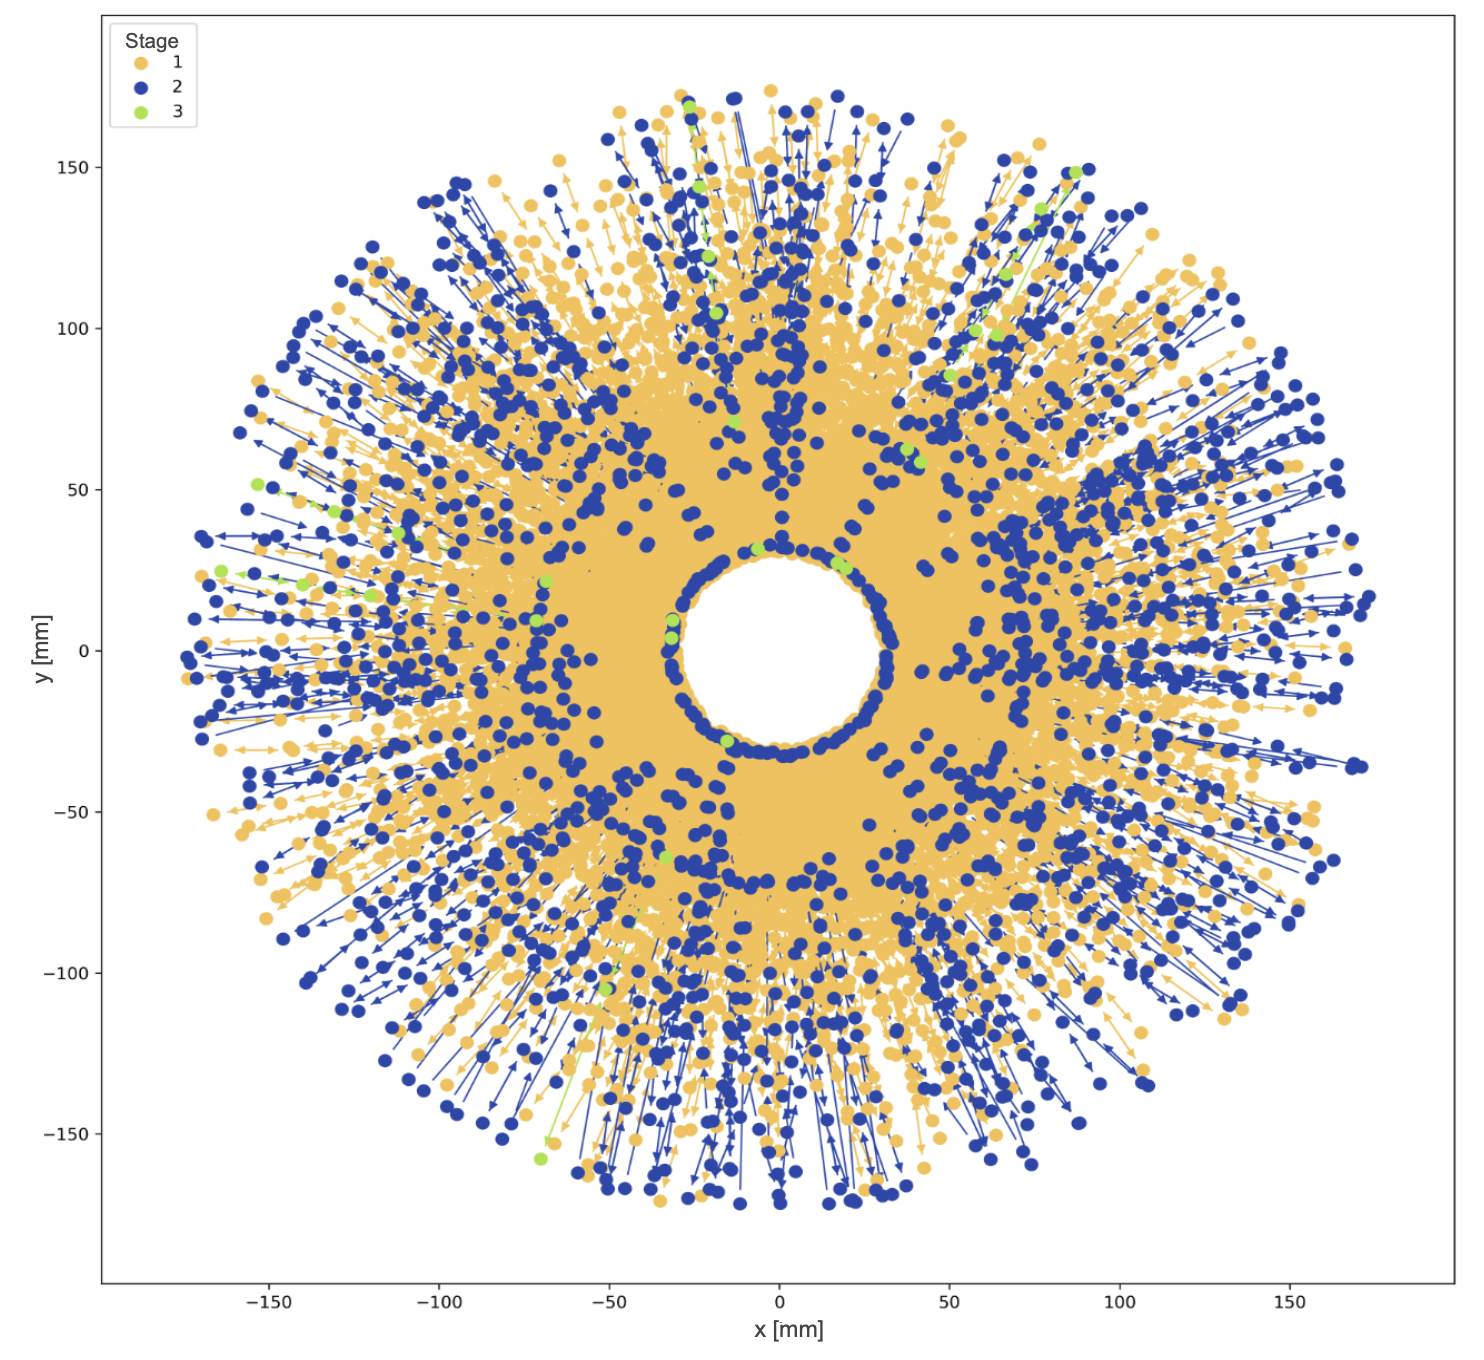
\includegraphics[width=10cm]{images/7-results/trackml-endcap-barrel-extracted-xy.png} } \label{fig:trackml-results-barrel-endcap-extracted-xy}}%
    \hfill
    %\qquad
    \subfloat[\centering $r$-$z$ plane view]{{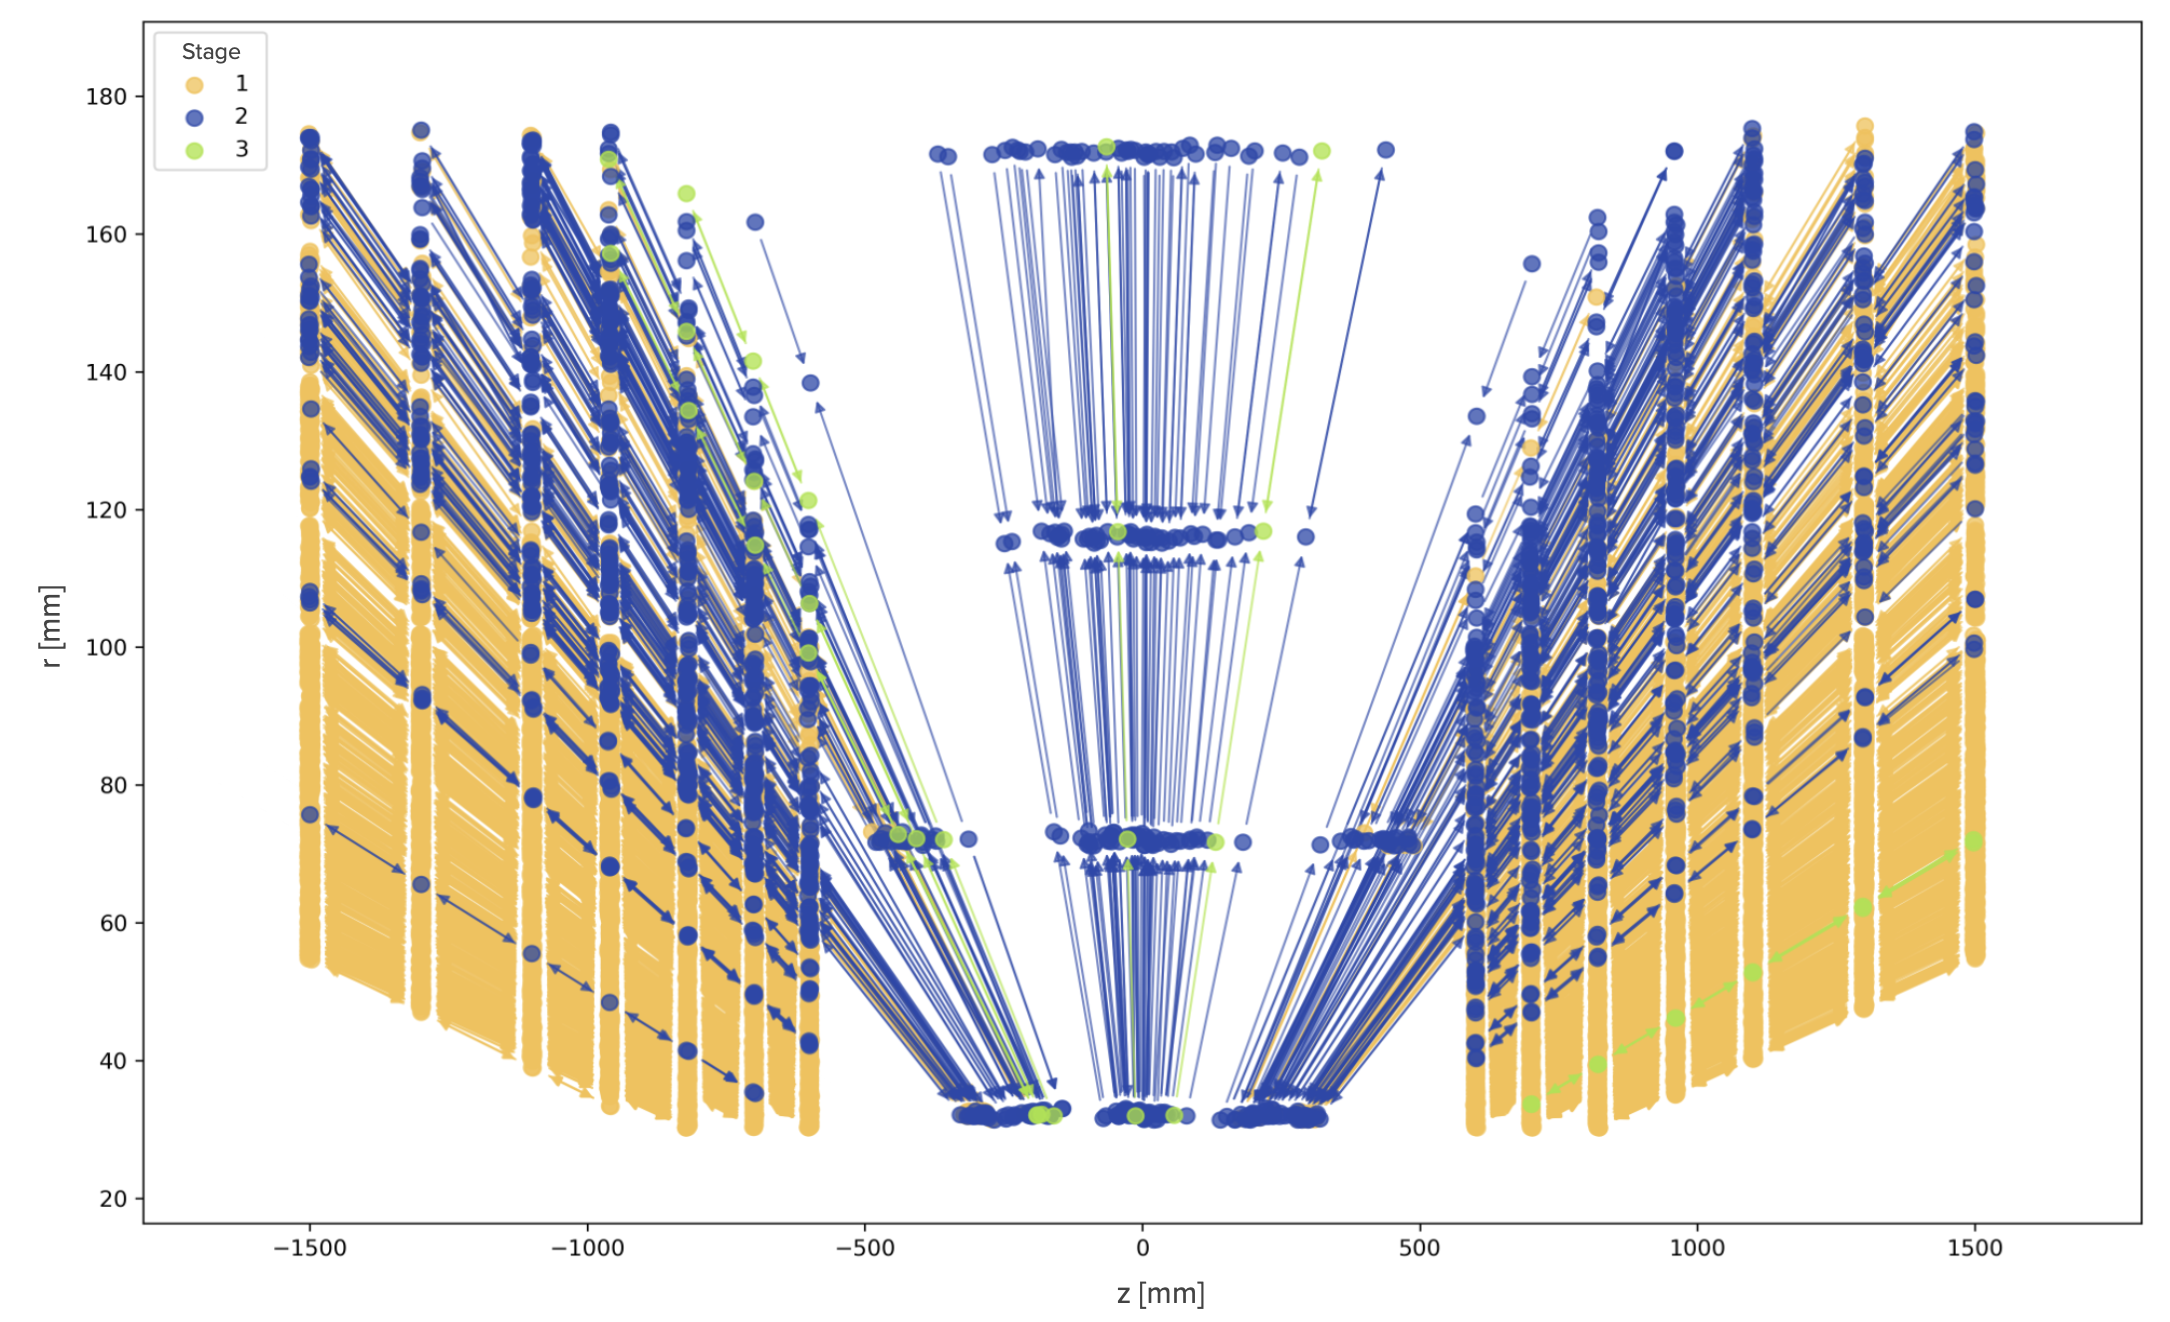
\includegraphics[width=14.5cm]{images/7-results/trackml-endcap-barrel-extracted-rz.png} } \label{fig:trackml-results-barrel-endcap-extracted-rz}}%
    \caption{Extracted track candidates post application of the iterative GNN algorithm onto the Pixel detector of the TrackML model.}%
    \label{fig:trackml-results-barrel-endcap}%
\end{figure}










\begin{figure}[htbp]
    \centering
    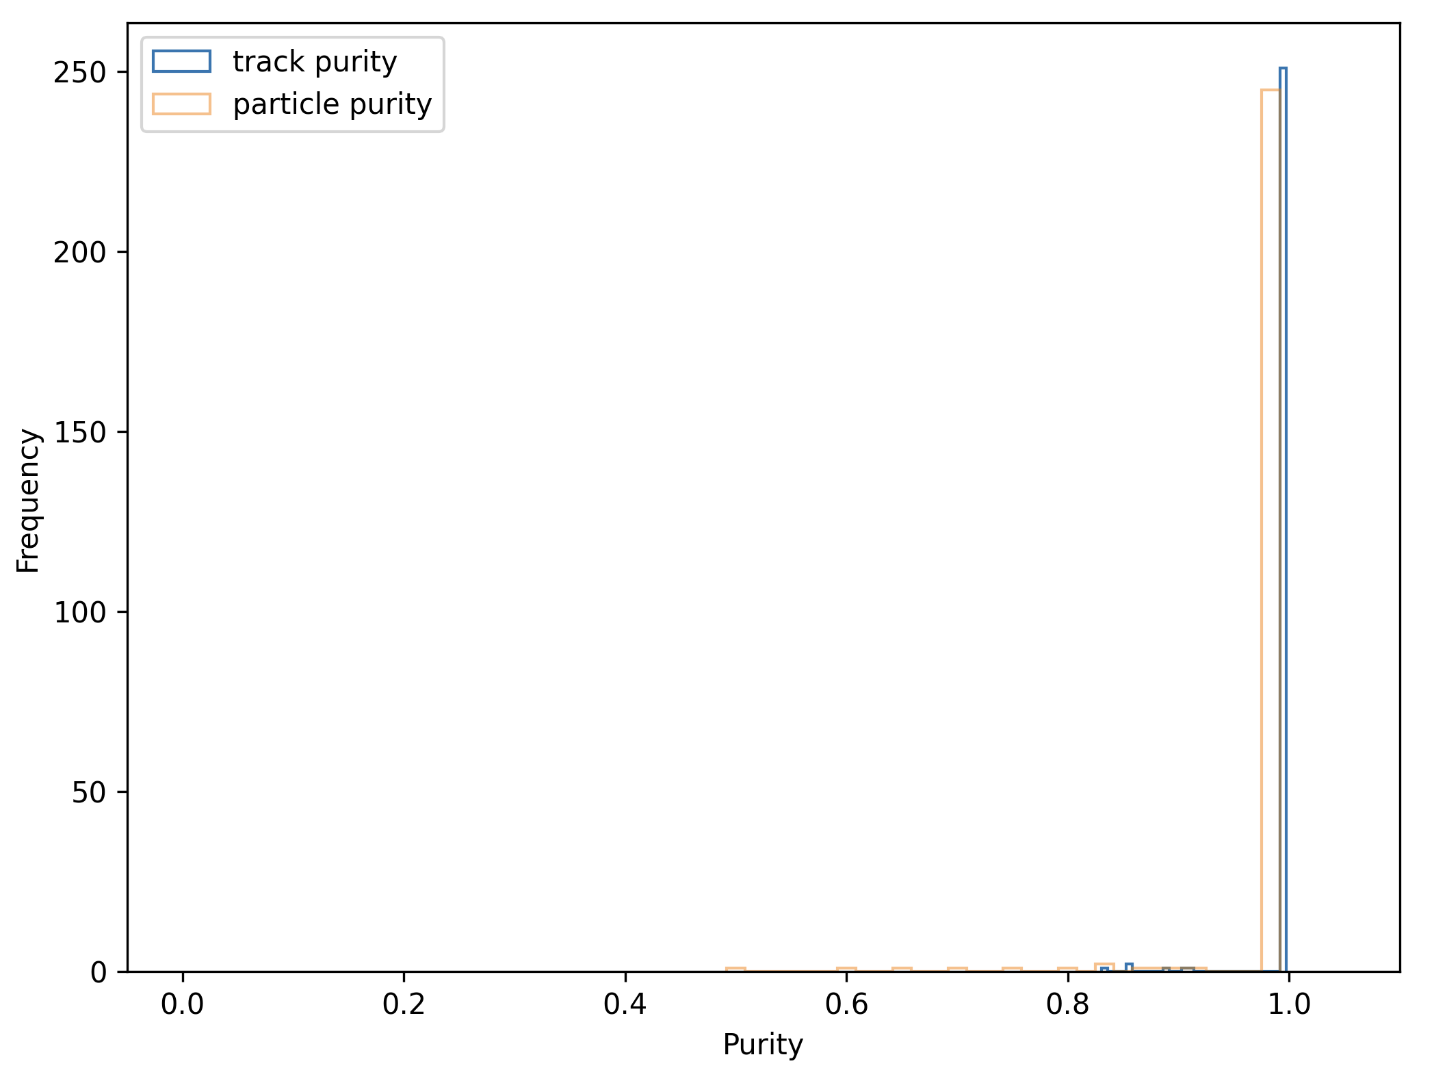
\includegraphics[width=0.7\textwidth]{images/7-results/barrel-and-endcap-purity.png}
    \caption{...}
    \label{fig:trackml-results-barrel-endcap-purity}%
\end{figure}



\subsubsection{Confusion Matrices}

% confusion matrices for barrel and endap, stages 1 and 2
\begin{figure}
    \centering
    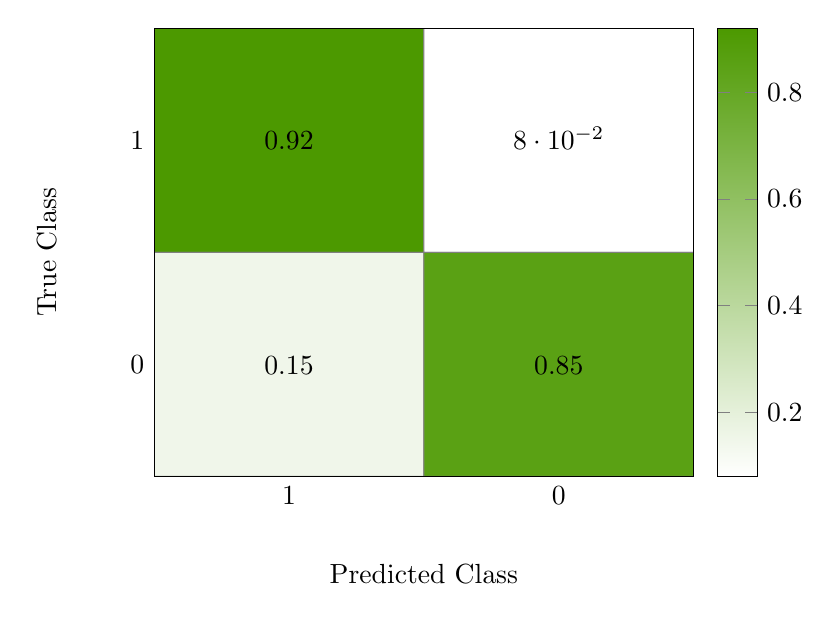
\begin{tikzpicture}
        \begin{axis}[
                colormap={greenyellow}{color=(white) rgb255=(76,153,0)},
                xlabel=Predicted Class,
                xlabel style={yshift=-15pt},
                ylabel=True Class,
                ylabel style={yshift=20pt},
                xticklabels={1, 0}, % changed
                xtick={0,...,1}, % changed
                xtick style={draw=none},
                yticklabels={1, 0}, % changed
                ytick={0,...,1}, % changed
                ytick style={draw=none},
                enlargelimits=false,
                colorbar,
                xticklabel style={rotate=0},
                nodes near coords={\pgfmathprintnumber\pgfplotspointmeta},
                nodes near coords style={yshift=-7pt},
            ]
            \addplot[
                matrix plot,
                mesh/cols=2, % changed
                point meta=explicit,draw=gray
            ] table [meta=C] {
                x y C
                0 0 0.92
                1 0 0.08     
                0 1 0.15
                1 1 0.85
            };
        \end{axis}
    \end{tikzpicture}
    \caption{Confusion matrix for Stage 1 of the GNN algorithm applied to the Pixel barrel and endcap of the TrackML detector model.}
    \label{fig:confusion-matrix-barrel-endcap-stage-1}
\end{figure}


\begin{figure}
    \centering
    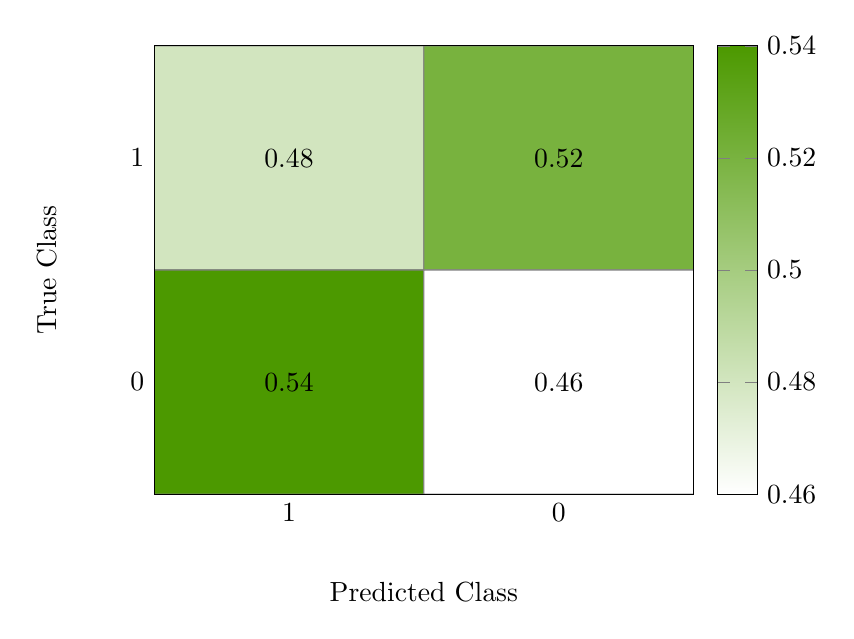
\begin{tikzpicture}
        \begin{axis}[
                colormap={greenyellow}{color=(white) rgb255=(76,153,0)},
                xlabel=Predicted Class,
                xlabel style={yshift=-15pt},
                ylabel=True Class,
                ylabel style={yshift=20pt},
                xticklabels={1, 0}, % changed
                xtick={0,...,1}, % changed
                xtick style={draw=none},
                yticklabels={1, 0}, % changed
                ytick={0,...,1}, % changed
                ytick style={draw=none},
                enlargelimits=false,
                colorbar,
                xticklabel style={rotate=0},
                nodes near coords={\pgfmathprintnumber\pgfplotspointmeta},
                nodes near coords style={yshift=-7pt},
            ]
            \addplot[
                matrix plot,
                mesh/cols=2, % changed
                point meta=explicit,draw=gray
            ] table [meta=C] {
                x y C
                0 0 0.48
                1 0 0.52     
                0 1 0.54
                1 1 0.46
            };
        \end{axis}
    \end{tikzpicture}
    \caption{Confusion matrix for Stage 1 of the GNN algorithm applied to the Pixel barrel and endcap of the TrackML detector model.}
    \label{fig:confusion-matrix-barrel-endcap-stage-2}
\end{figure}





\subsection{Execution Times}



\subsubsection{Remaining Network Post Track Extraction}



\begin{figure}[htbp]
    \centering
    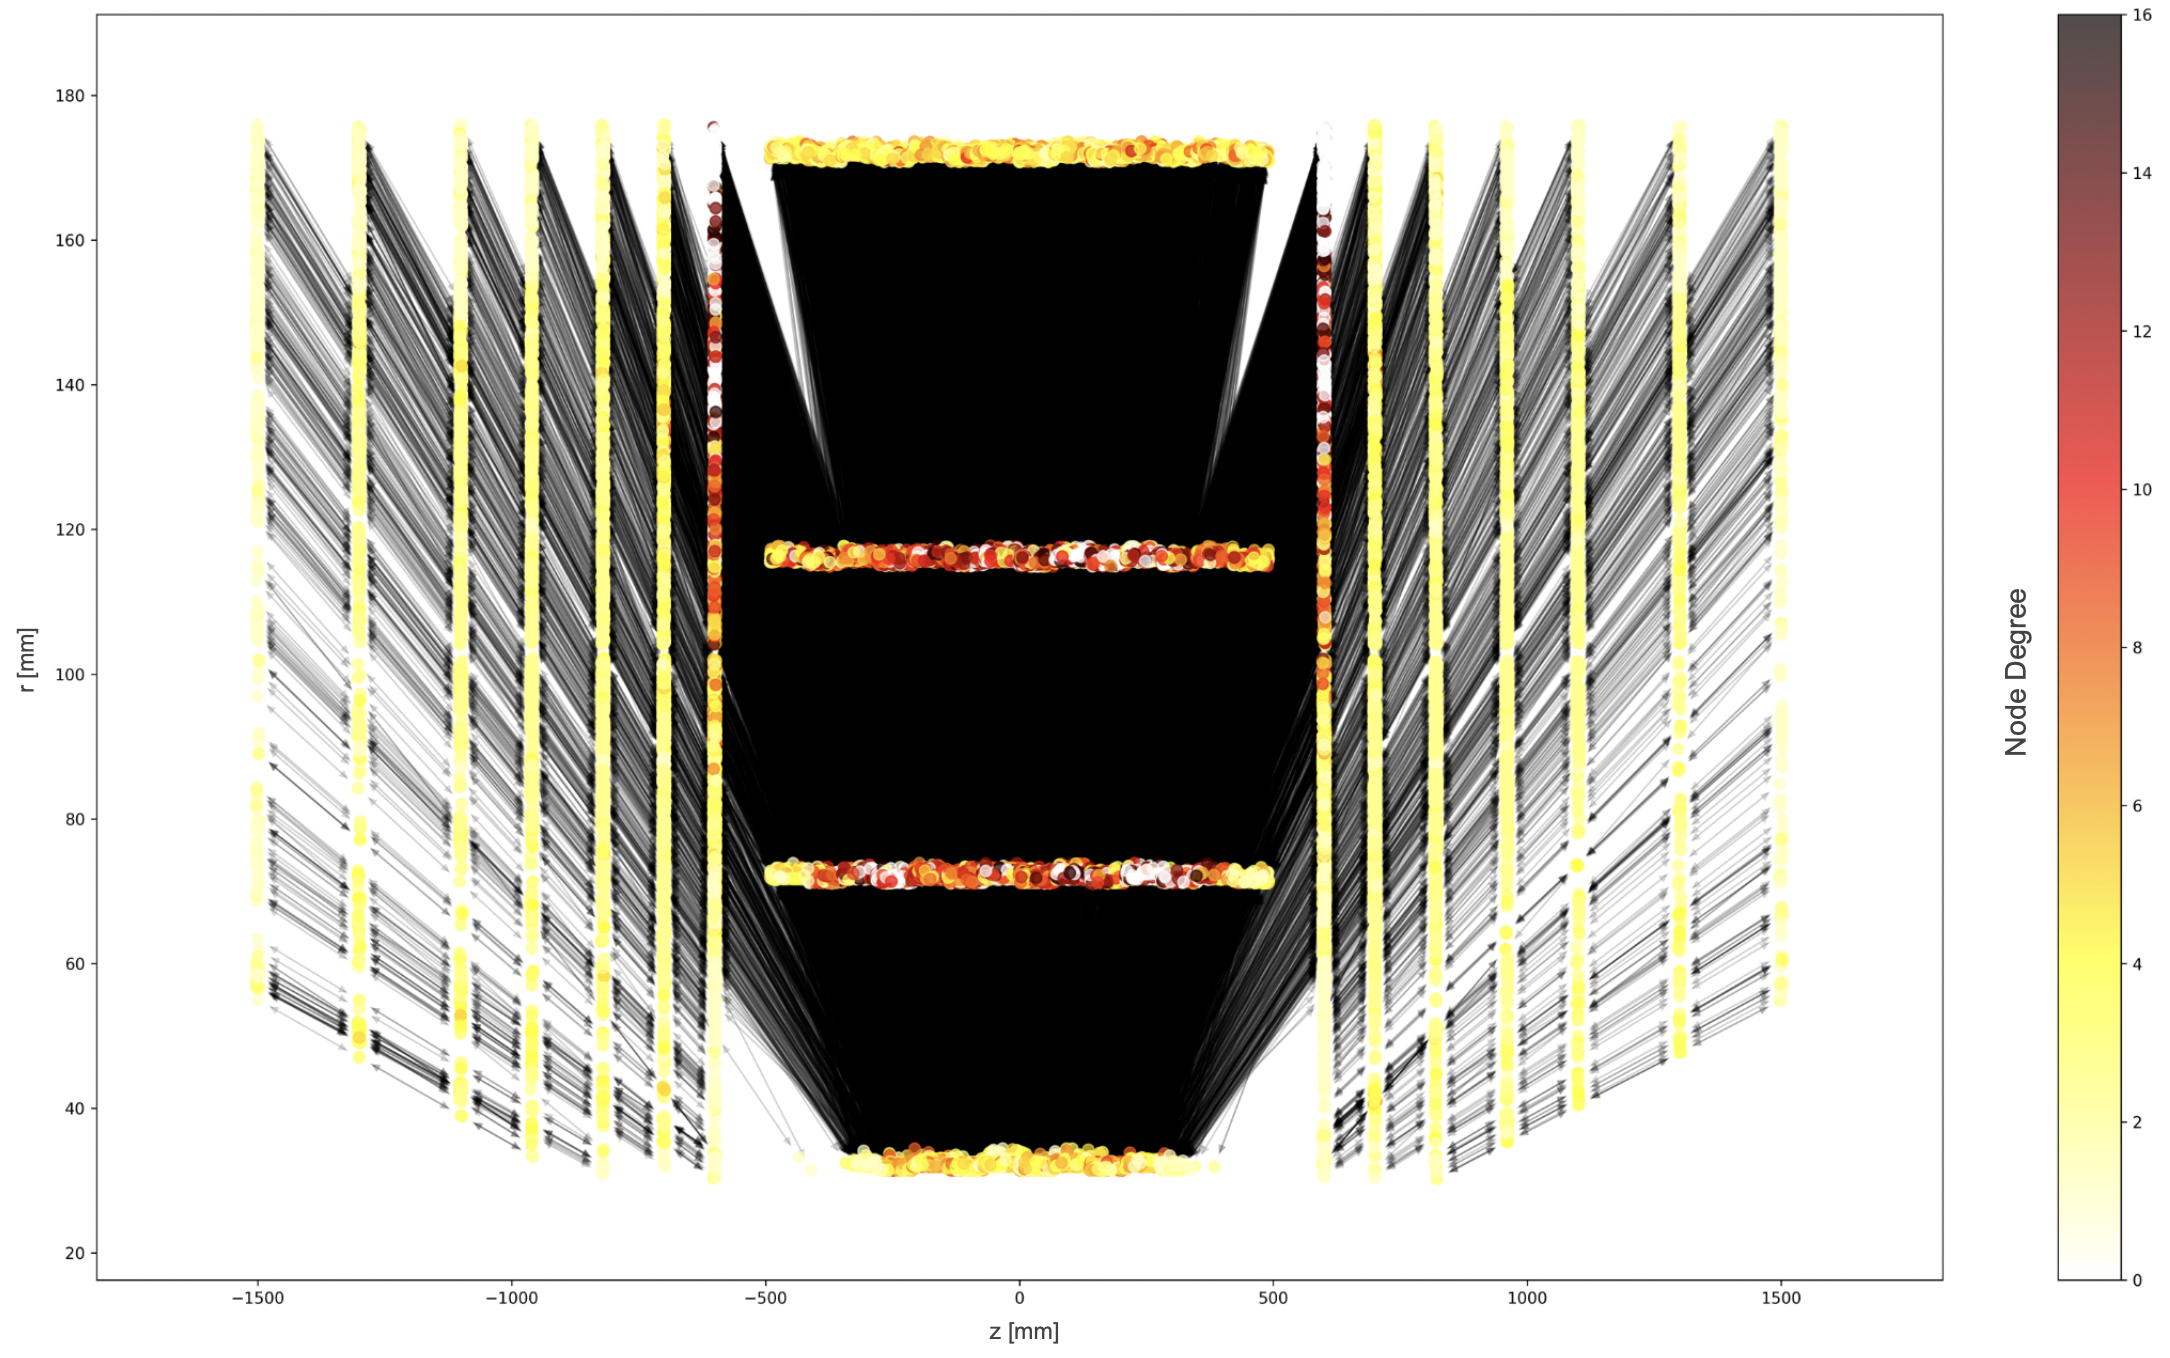
\includegraphics[width=0.99\textwidth]{images/7-results/trackml-barrel-remaining-node-degree.png}
    \caption{TODO: regenerate this plot but with the node degree inverted!!! }
    \label{fig:trackml-results-barrel-endcap-remaining-node-degree}%
\end{figure}


\subsubsection{Improvement in KF for Extrapolation in r-z plane}

- 4 different scenarios, barrel to barrel, endcap to barrel etc etc for the r-z plane







\subsection{Software Optimisations}


The following improvements are necessary for proper online usage in detector experiments.

% improvements to implementation - numpy matrices for everything, potential GPU accelerated calculations, improvements to the graph network initialisation stage

% Discuss possible computational refinements and improvements and this can be implemented for proper online usage in detectors

%Mention GPU implementation, one can use possibly QuPy library for optimised numpy and provide a link to this (website)





\subsection{Other Approaches}
\subsubsection{Community Detection}

If a subgraph does not meet the criteria to qualify as a good track candidate outlined in Section \ref{gnn-track-extration}, a technique known as \textit{Community Detection} \cite{community} is applied in order to further partition the set of nodes. Community Detection is a generalisation of CCA and works by using a distance metric, typically modularity, in order to label nodes into groups such that all nodes in a group are \textit{closely connected}. Modularity is a benefit function that measures the strength of a particular division of a network using the number of edges and edge weights. A popular modularity maximisation approach is the Louvain method \cite{python_louvain}, which iteratively optimises local communities until global modularity can no longer be improved. An example illustration of a network partition via Community Detection using modularity is shown in Figure \ref{fig:community-detection}. 

\begin{figure}[htbp!] 
    \centering
    \subfloat[]{%
        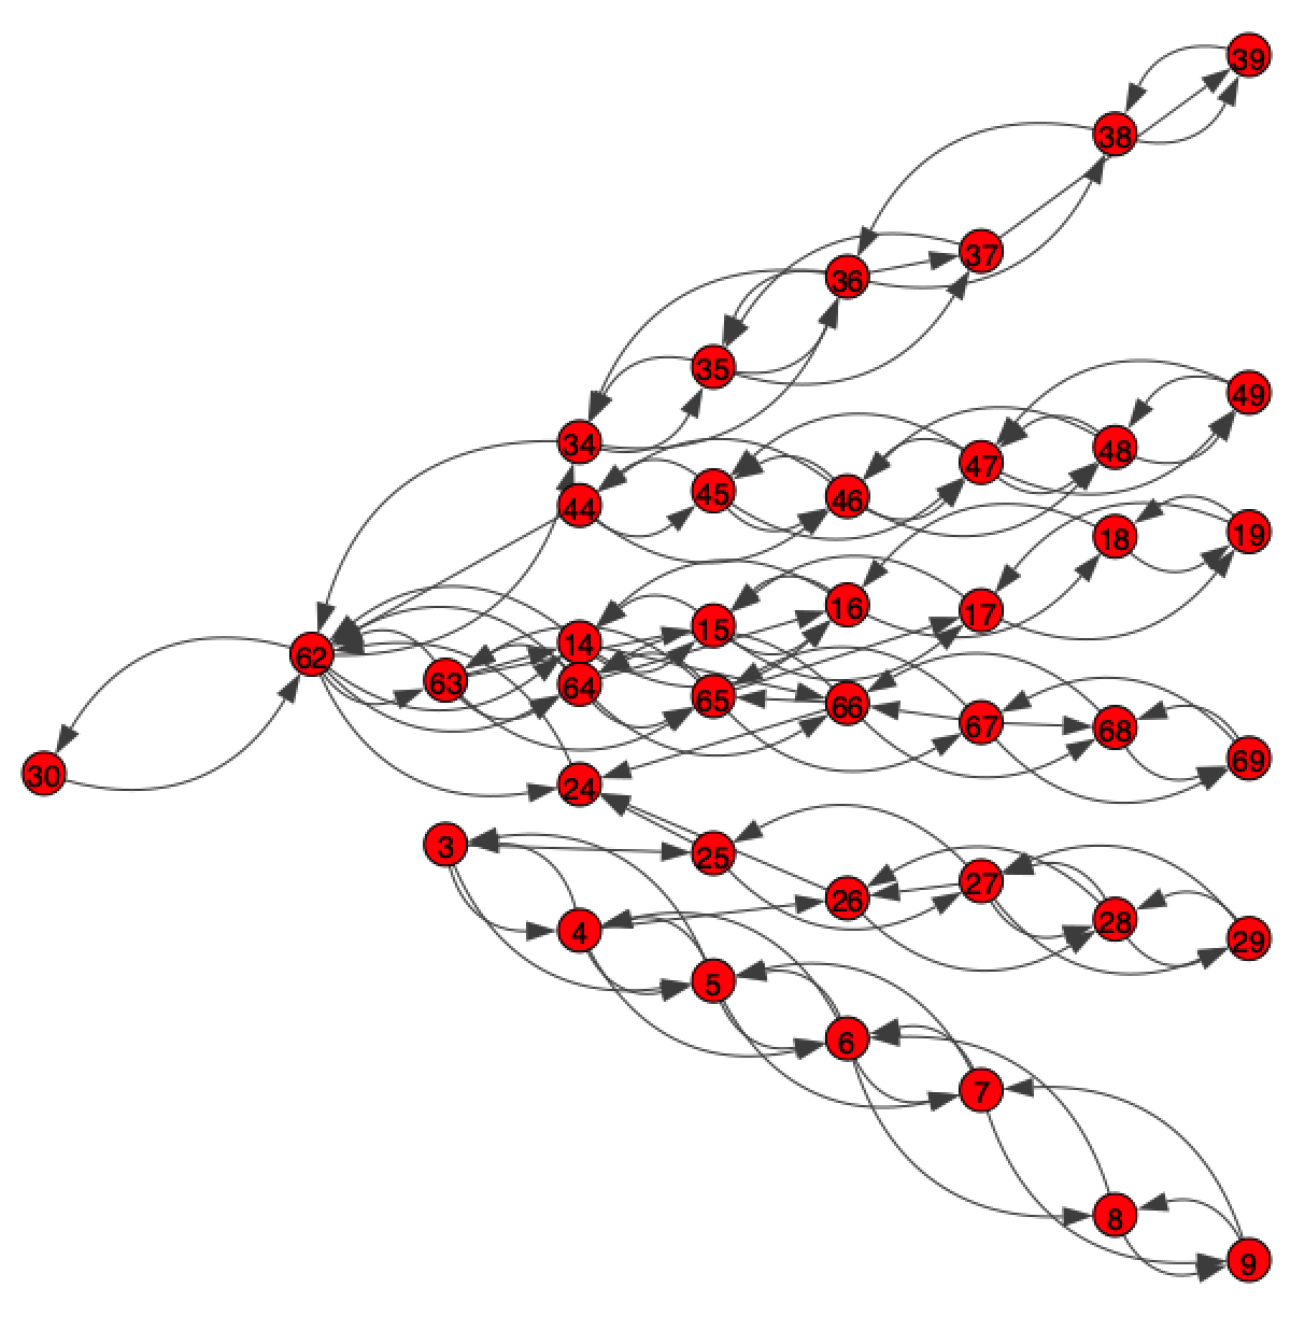
\includegraphics[width=0.45\linewidth]{images/7-results/community-detection-1.png}%
        \label{fig:community-detection-1}%
        }%
    \hfill%
    \subfloat[]{%
        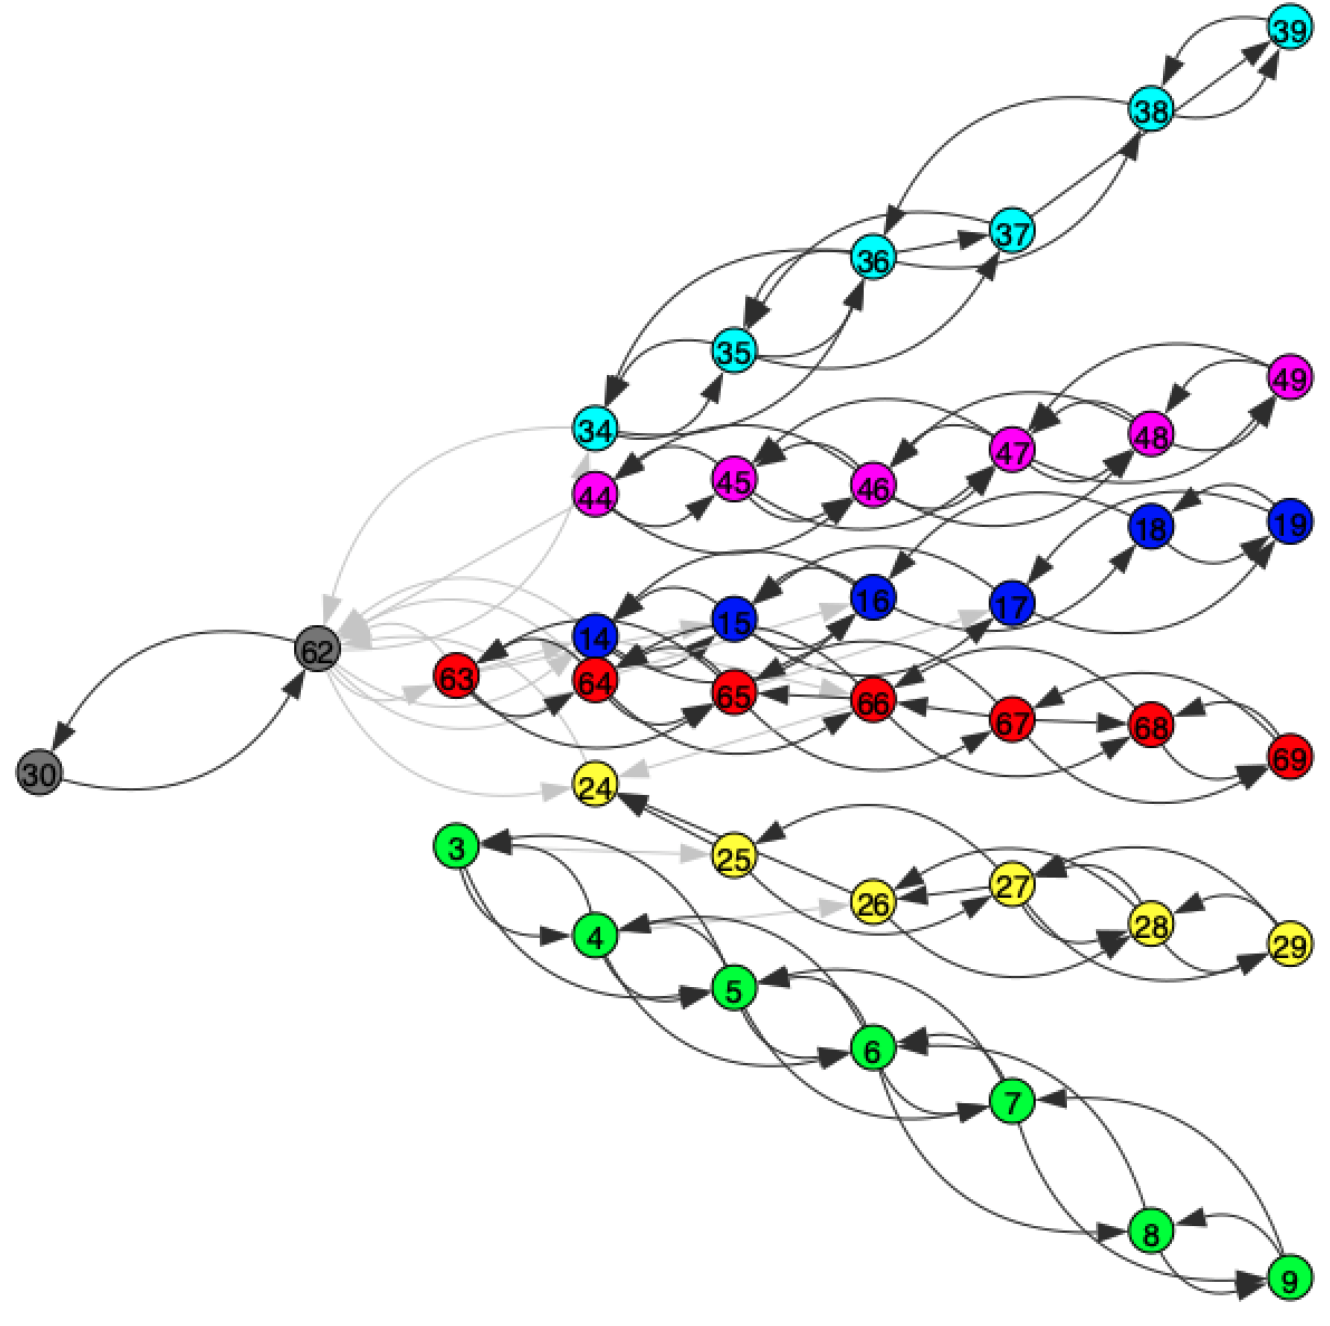
\includegraphics[width=0.45\linewidth]{images/7-results/community-detection-2.png}%
        \label{fig:community-detection-2}%
        }%
    \caption{Example application of the Community Detection algorithm applied to a small group of nodes from a TrackML event. a) Subset of nodes and edges connected as one subgraph shown in red. b) Post application of the Community Detection algorithm. Separation of the subgraph in a) into potential track candidates represented by separate colours. The faint grey edges show connections that have been deactivated through Community Detection.}
    \label{fig:community-detection}
\end{figure}

Figure \ref{fig:community-detection-1} shows a small subset of nodes from a TrackML event and its corresponding edges connected as one subgraph. The general shape of the network shows the tracks originating from the left-hand side and their trajectories move towards the right-hand side. The results of application of Community Detection are shown in Figure \ref{fig:community-detection-2}. In this instance, the Community Detection was successful to partition the network into a total of seven subgraphs shown by separate colours. Six of these subgraphs met the criteria for a good track candidate, and a single track fragment was also formed shown by the grey subgraph containing two nodes. However upon further investigation, this procedure did not work successfully in all cases, specifically in dense environments, and the algorithm was found to not utilize node properties during network partition. Therefore, as this procedure needed further refinement, it was not implemented into the main GNN pattern recognition algorithm. 

A technique such as Community Detection is advantageous for a problem such as track splitting, as it provides fast convergence in track extraction, given that the algorithm is adapted for highly dense environments.





\section{Conclusion}

% Good to see that the GNN algorithm works on an event with significant track multiplicity

% Utilizing message passing to iteratively learn neighbourhood information aids in the pruning of outlier edges within complex regions.

% This key feature of the GNN-based algorithm suggests that the excitation and inhibition rules of individual GNN nodes are designed in such a way to facilitate the “simple-to-complex” approach for “nodes-to-tracks” association. 

% The approach developed here is a novel method using a GNN-based framework for track finding, unlike the traditional approach whereby Multi-Layered Perceptrons are trained to directly classify nodes and edges. By utilising various machine learning techniques, the graph network is allowed to learn local track parameters on its own by iteratively resolving ambiguities and discover track candidates. The main stages of the algorithm comprise of a Gaussian Mixture Reduction stage and neighbourhood information aggregation stage. The use of Kalman filters for both information aggregation and track extraction embedded into the network is a novel approach and has shown to successfully extract track candidates compatible with the particle motion model. The algorithm yields promising results on both a simple MC toy model and TrackML model for the endcap region. A preliminary result of $>$ 90\% track reconstruction efficiency is achieved for fully contained tracks within the endcap volume and with $p_{T} >$ 1GeV. It is promising to see that this methodology provides a high performance on a small dataset, however the algorithm is still within the early stages of its development. An evaluation on the Pixel barrel of the TrackML dataset is a work in progress, as well as within denser hit environments in order to sufficiently assess the quality of the algorithm. 